\documentclass[12pt,a4paper]{article}
\usepackage[a4paper,total={160mm,250mm}]{geometry}
\usepackage[utf8]{inputenc}
\usepackage[ruled,vlined]{algorithm2e}
\usepackage{amsmath}
\usepackage{amsthm}
\usepackage{amsfonts}
\usepackage{amssymb}
\usepackage{amscd}
\usepackage{array}
\usepackage{caption}
\usepackage{dirtree}
\usepackage{enumitem}
\usepackage{graphicx}
\usepackage[colorlinks=true,linkcolor=blue]{hyperref}
\usepackage{minted}
\usepackage{mathtools}
\usepackage{mdframed}
\usepackage{ngerman}
\usepackage{subcaption}
\usepackage{tcolorbox}
\usepackage{tikz}
\usepackage{xcolor}
%\usepackage[inline]{showlabels}

\tcbuselibrary{breakable}

\definecolor{shade}{gray}{.5}

\renewcommand*{\thesection}{\arabic{section}}
\renewcommand{\thesubfigure}{\roman{subfigure}}

%\theoremstyle{definition}
%\newtheorem{aufgabe}{Aufgabe}
%\numberwithin{aufgabe}{section}
%\theoremstyle{definition}
%\newtheorem*{losung}{Lösung}

\newcounter{taskcounter}
\numberwithin{taskcounter}{section}

\newenvironment{aufgabe}{%
	\refstepcounter{taskcounter}
	\mdfsetup{%
		frametitle={%
			\tikz[baseline=(current bounding box.east),outer sep=0pt]
			\node[anchor=east,rectangle,fill=blue!20]
			{\strut Aufgabe~\thetaskcounter};
		}
	}
	\mdfsetup{%
		innertopmargin=5pt,linecolor=blue!20,%
		linewidth=2pt,topline=true,roundcorner=5pt,%
		frametitleaboveskip=\dimexpr-\ht\strutbox\relax%
	}
	\begin{mdframed}[nobreak=false]\relax
}{%
	\end{mdframed}
}

\newenvironment{losung}{%
	\mdfsetup{%
		frametitle={%
			\tikz[baseline=(current bounding box.east),outer sep=0pt]
			\node[anchor=east,rectangle,fill=green!20]
			{\strut Lösung};
		}
	}
	\mdfsetup{%
		innertopmargin=5pt,linecolor=green!20,%
		linewidth=2pt,topline=true,roundcorner=5pt,%
		frametitleaboveskip=\dimexpr-\ht\strutbox\relax%
	}
	\begin{mdframed}[nobreak=false]\relax
}{%
	\end{mdframed}
}

%\newtcolorbox{mybox}[3][]
%{
%	colframe = #2!25,
%	colback  = #2!10,
%	coltitle = #2!20!black,  
%	title    = {#3},
%	#1,
%}
%\newcounter{taskcounter}
%\numberwithin{taskcounter}{section}
%\newenvironment{aufgabe}{%
%	\refstepcounter{taskcounter}
%	\begin{mybox}{blue}{Aufgabe~\thetaskcounter}\relax
%	}{%
%	\end{mybox}
%}
%\newenvironment{losung}{%
%	\begin{mybox}{red}{Lösung}\relax
%	}{%
%	\end{mybox}
%}

%\pagestyle{empty}
\makeatletter\@addtoreset{section}{part}\makeatother%

\title{Eigengesichter}
\author{Oliver Rietmann}
\date{\today}

\begin{document}
\begin{titlepage}
	{\hspace{-1cm}
\includegraphics[width=0.3\textwidth]{images/ETHlogo}\par}
	\vspace{1cm}
	\begin{center}
	{\scshape Mentorierte Arbeit in Fachdidaktik Mathematik\par}
	\vspace{1cm}
	{\large\bfseries Eigengesichter\par}
	\vspace{1cm}
	{Oliver Rietmann\par}
	\vfill
	\end{center}
	{\bfseries Inhalt\par}
	{In dieser Arbeit wird die Technik der \textit{Eigengesichter} (engl. \textit{eigenfaces}) erklärt. Hierbei handelt es sich um eine rudimentäre Methode zur Gesichtserkennung, welche durch Computer automatisiert werden kann. Unter Gesichtserkennung versteht man klassischerweise das (automatisierte) identifizieren einer Person auf einem Foto. Aber auch damit verwandte Aufgaben werden hier besprochen.
	Diese Arbeit führt die Leser durch eine Anleitung zur Implementierung eines solchen Programms in Python. Der Fokus liegt dabei auf der zugrundeliegenden Mathematik dieses Verfahrens. Die dazu verwendeten Unterrichtsmethoden sollen zudem aus didaktischer Sicht beleuchtet werden.\par}
	\vspace{0.5cm}
	{\bfseries Zielpublikum\par}
	{Fortgeschrittene gymnasiale MittelschülerInnen mit Schwerpunkt Mathematik und StudentInnen einer mathematischen/technischer Fachrichtung.\par}
	\vspace{0.5cm}
	{\bfseries Voraussetzungen\par}
	{Vertrautheit mit den Grundbegriffen der linearen Algebra (Vektoren, Matrizen, Basis, Linearkombination, Unterräume von $\mathbb R^n$).
	Zudem werden grundlegende Programmierkenntnisse vorausgesetzt.\par}
	\vspace{0.5cm}
	{\bfseries Form\par}
	{Text mit Aufgaben, Lösungen und Lernzielen. Die Python-Codes befinden sich im Anhang. Alternativ können sie online heruntergeladen werden. (Der Link befindet sich in der Arbeit.)\par}
	\vspace{0.5cm}
	{\bfseries Betreuung\par}
	{Christian Rüede\par}
	\vspace{0.5cm}
	{\bfseries Datum\par}
	{\today\par}
\end{titlepage}
%\maketitle
\tableofcontents
\clearpage
\part{Lernskript: Eigengesichter}
Historisch gesehen war die Methode der Eigengesichter das erste durch Computer automatisierbare Verfahren zur Gesichtserkennung.
Das Fundament dazu wurde 1987 durch Sirovich and Kirby entwickelt \cite{SirovichKirby1987}.
In ihrer Arbeit verwendeten Sie bereits den Begriff \textit{eigenpictures}.
Sie zeigten auf, wie man Fotos von Gesichtern geeignet durch Begriffe der linearen Algebra beschreiben kann.
Damit war der Weg frei um die mächtige Maschinerie der Mathematik, insbesondere der linearen Algebra und der Statistik, auf Fotos anzuwenden.
Dies geschah schon kurz darauf, nämlich 1991, durch Turk und Pentland \cite{Turk1991}.
Sie verwendeten bereits den Begriff \textit{eigenfaces} und beschrieben das Verfahren zur Gesichtserkennung, welches auch wir implementieren werden.
Modernere Methoden wie zum Beispiel \textit{DeepFace} von Facebook funktionieren allerdings viel besser als unsere rudimentäre Methode und sind so gut wie echte Menschen bei der Gesichtserkennung \cite{Taigman2014}.
Ein Vergleich der (heutzutage) besten Methoden findet man zum Beispiel hier \cite{Taskiran2020}.

Alle solchen Programme, auch die modernsten, verwenden eine \textit{Datenbank} von Bildern von Gesichtern, deren Identität bereits bekannt ist.
Man hat also eine gewisse Anzahl von Personen.
Jeder einzelnen Person sind mehrere Bilder zugeordnet, nämlich die Bilder, welche das Gesicht eben dieser Person zeigen.
Man kann sich das als Unterteilung in verschiedene Klassen vorstellen: Zu jeder Person gehört eine Klasse und jede Klasse enthält eine Menge von Bildern.
Dies ist in Abbildung~\ref{fig:database} veranschaulicht.
\begin{figure}[ht]
	\centering
	\begin{tabular}{l m{2cm} m{2cm} m{2cm} m{2cm} c}
		\textbf{Klasse (Person)} & \textbf{Bild 1} & \textbf{Bild 2} & \textbf{Bild 3} & \textbf{Bild 4} & $\cdots$ \\ \hline
		Adam Sandler & 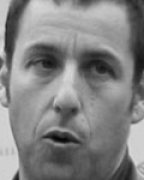
\includegraphics[width=0.1\textwidth]{images/intro/class0_0} &
		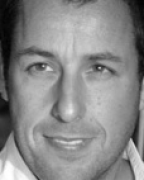
\includegraphics[width=0.1\textwidth]{images/intro/class0_1} & 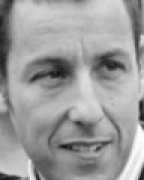
\includegraphics[width=0.1\textwidth]{images/intro/class0_2} & 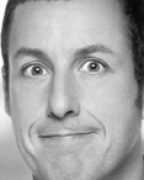
\includegraphics[width=0.1\textwidth]{images/intro/class0_3} & $\cdots$ \\ \hline
		Emma Watson & 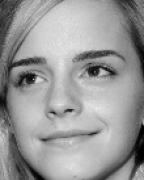
\includegraphics[width=0.1\textwidth]{images/intro/class1_0} &
		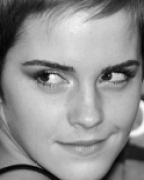
\includegraphics[width=0.1\textwidth]{images/intro/class1_1} & 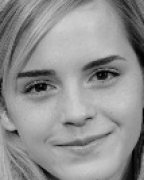
\includegraphics[width=0.1\textwidth]{images/intro/class1_2} & 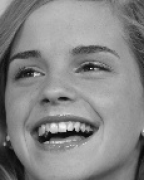
\includegraphics[width=0.1\textwidth]{images/intro/class1_3} & $\cdots$ \\ \hline
		Natalie Portman & 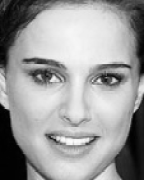
\includegraphics[width=0.1\textwidth]{images/intro/class2_0} & 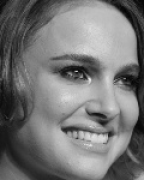
\includegraphics[width=0.1\textwidth]{images/intro/class2_1} & 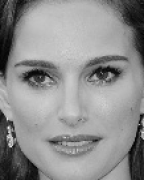
\includegraphics[width=0.1\textwidth]{images/intro/class2_2} & 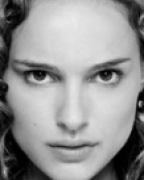
\includegraphics[width=0.1\textwidth]{images/intro/class2_3} & $\cdots$ \\ \hline
		$\qquad\qquad\vdots$ & $\qquad\vdots$ & $\qquad\vdots$ & $\qquad\vdots$ & $\qquad\vdots$ & $\ddots$ \\
	\end{tabular}
	\caption{Visualisierung einer Datenbank von Bildern von Gesichtern.}
	\label{fig:introduction}
\end{figure}
Aus dieser Datenbank \glqq{}lernt\grqq{} das Programm, neue Bilder zu klassifizieren, also den Personen aus der Datenbank zuzuordnen.
Das Wort \glqq{}neu\grqq{} bedeutet hier, dass dieses Bild nicht notwendigerweise in der Datenbank enthalten ist.
Die Person auf dem Bild muss aber in der Datenbank sein!
Würde die Datenbank in Abbildung~\ref{fig:introduction} wirklich nur diese drei Personen enthalten, so könnte man zum Beispiel kein Bild von Brad Pitt korrekt klassifizieren, auch wenn eine noch so gute Methode verwendet wird.
Die Datenbank und die Methode der Gesichtserkennung sind unabhängig voneinander.
Das heisst einerseits, aus der selben Datenbank können verschiedene Methoden lernen.
Andererseits kann ein und die selbe Methode verschiedene Datenbanken nutzen.
Wie gut die Gesichtserkennung am Schluss funktioniert hängt nicht nur von der Methode selbst ab, sondern auch von der Datenbank, welche diese verwendet.
Grundsätzlich gilt, dass jede Methode umso besser funktioniert, je mehr Bilder pro Person in der Datenbank gespeichert sind, die sie verwendet.
Mit \glqq{}gut funktionieren\grqq{} ist gemeint, dass neue Bilder mit hoher Wahrscheinlichkeit richtig klassifiziert werden.

Die in Abbildung~\ref{fig:introduction} gezeigten Bilder stammen aus einer Datenbank von über 10'000 Bildern von über 100 berühmten Persönlichkeiten \cite{Chen14}.
Die Bilder sind alle schwarz-weiss und zeigen lediglich die Gesichter der Personen.
Genau diese Datenbank werden wir auch für alle nachfolgenden Kapitel verwenden.
Sie ist unter folgendem Link zu finden:
\begin{center}
	\url{https://people.math.ethz.ch/~rioliver/eigenfaces/datenbank.zip}
\end{center}
Allerdings kann auch eine andere Datenbank verwendet werden, sofern sie in das richtige Format gebracht wird.
Eine Anleitung dazu befindet sich in Kapitel~\ref{sec:database}.

Das Grundgerüst eines Programms zur Gesichtserkennung in Python steht uns schon zur Verfügung.
Wir werden dieses in den folgenden Kapiteln zu einem voll funktionsfähigen Programm erweitern.
Der gesamte Code befindet sich auf GitHub und kann unter folgendem Link heruntergeladen werden:
\begin{center}
	\url{https://github.com/OliverRietmann/eigenfaces}
\end{center}
\section{Datenbank einrichten} \label{sec:database}
Bitte laden Sie nun die Datenbank herunter (mit dem Link aus der Einleitung) und entpacken Sie diese.
Wir nennen das entstehende Verzeichnis \texttt{datenbank}.
Laden Sie ebenfalls die Python-Codes herunter.
Führen Sie als erstes das Python-Skript \texttt{save\_eigenfaces.py} über die Kommandozeile (Linux, MacOS) oder über \href{https://ipython.org/install.html}{IPython} (Windows) aus und übergeben Sie dabei den Pfad zur Datenbank und einen Namen für das resultierende File (z.B. \texttt{eigenfaces.dat}), also
\begin{center}
\mintinline{python}{python3 save_eigenfaces.py datenbank eigenfaces.dat}
\end{center}
Dies generiert ein File \texttt{eigenfaces.dat} welches wir später brauchen um die Aufgaben zu lösen.
Damit lassen sich alle nachfolgenden Kapitel bearbeiten.
Alternativ kann man eine eigene Datenbank erstellen und stattdessen diese für die Bearbeitung des Lernskriptes verwenden.
Dieses Kapitel ist eine Anleitung dazu.
Es werden folgende Programme benötigt:
\begin{itemize}
	\item Ein Bildbearbeitungsprogramm wie zum Beispiel das open source Programm \href{https://www.gimp.org/}{GIMP}.
	\item Ein Tabellen-Kalkulationsprogramm wie zum Beispiel das open source Programm \href{https://de.libreoffice.org/discover/calc/}{LibreOffice Calc}.
\end{itemize}
Nehmen wir als Beispiel eine Schulklasse bestehend aus 10 Lernenden.
Jeder Schüler und jede Schülerin macht einige Fotos von seinem/ihrem Gesicht.
Sagen wir, 8 Fotos pro Person.
Das Ziel ist ein Verzeichnis \texttt{datenbank} anzulegen, welches wie in Abbildung~\ref{fig:database} aufgebaut ist.
\begin{figure}[ht]
	\centering
	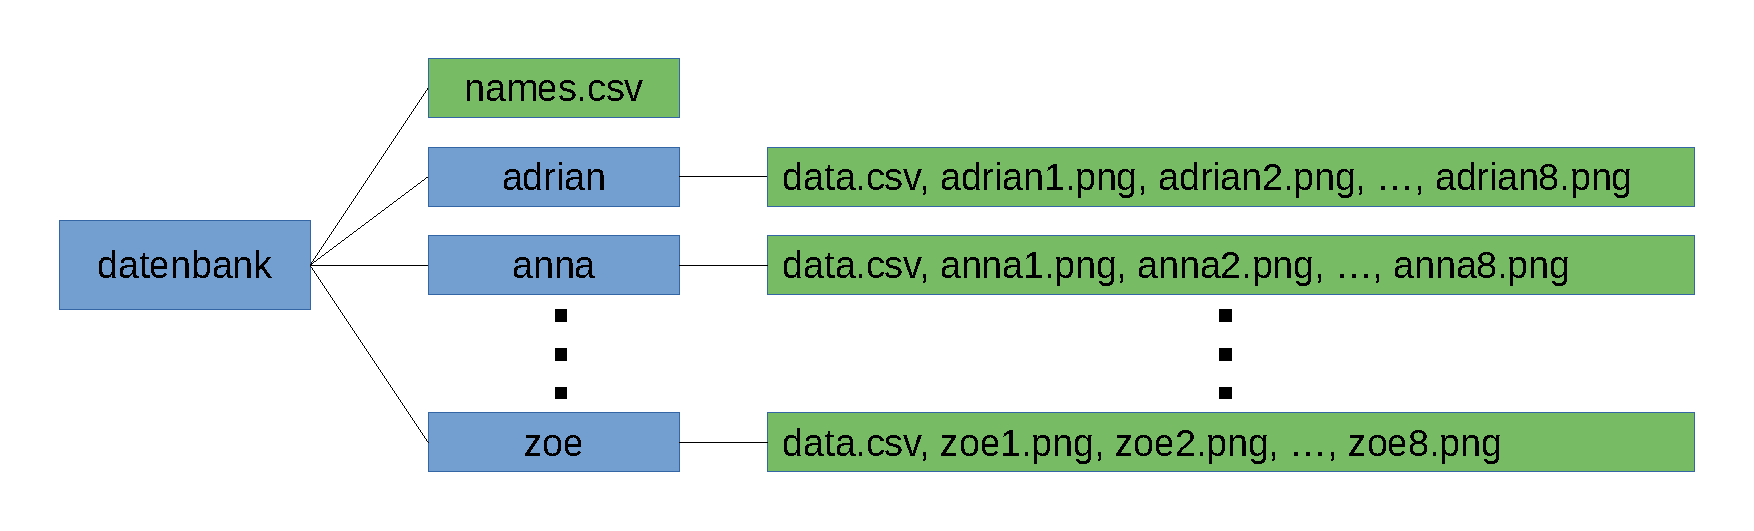
\includegraphics[width=\textwidth]{images/database}
	\caption{Datenbank aus Trainingsbildern. Die Verzeichnisse sind in blau und die Dateien in grün abgebildet.}
	\label{fig:database}
\end{figure}
Das heisst, pro Person enthält \texttt{datenbank} je ein Verzeichnis mit deren Namen.
Diese Verzeichnisse enthalten wiederum die 8 Fotos der jeweiligen Person.
Die Dateien mit der Endung \texttt{.csv} enthalten jeweils eine Tabelle und können mit einem Tabellenkalkulationsprogramm erstellt/editiert werden.
\begin{itemize}
	\item \texttt{names.csv}: Besteht aus 10 Zeilen, welche die 10 Unterverzeichnisse \texttt{adrian, anna, ..., zoe} von \texttt{datenbank} auflisten.
	Unser Programm benötigt dieses File um die Unterverzeichnisse zu finden.
	\item \texttt{data.csv}: Besteht aus 8 Zeilen, welche die Dateinamen der 8 Fotos auflisten.
	Zum Beispiel enthält \texttt{adrian/data.csv} die Zeilen \texttt{adrian1.png, adrian2.png, ..., adrian8.png}.
	Unser Programm benötigt dieses File um die Bilddateien in den Unterverzeichnissen zu finden.
\end{itemize}
Es fehlt noch ein letzter Schritt.
Die Bilder müssen noch in ein geeignetes Format gebracht werden.
Dazu verwenden wir ein Bildbearbeitungsprogramm.
\begin{itemize}
	\item Alle Bilder müssen auf die selbe Auflösung zugeschnitten werden.
	Eine geeignete Auflösung ist zum Beispiel eine Breite von $N=144$ Pixel und eine Länge von $M=180$ Pixel.
	\item Der vorherige Punkt sollte so bewerkstelligt werden, dass das Gesicht möglichst das ganze Bild ausfüllt.
	\item Alle Bilder müssen in ein schwarz-weiss Bild konvertiert werden.
\end{itemize}
Führen Sie dann die Schritte zu Beginn dieses Kapitels für diese Datenbank aus.

%\section{Eigengesichter} \label{sec:eigenfaces}
\begin{tcolorbox}
	\centerline{\textbf{Lernziele Kapitel~\ref{sec:facespace}}}
	\begin{enumerate}[leftmargin=*,label=\thesection.\arabic*]
		\item \label{item:distance} Die Lernenden können den Abstand eines Punktes von einer Gerade in höheren Dimensionen berechnen.\\
		(Aufgaben~\ref{aufg:distance_simple} und~\ref{aufg:distance_complex})
%		\item \label{item:eigenfaces} Die Lernenden verstehen die Konstruktion der Eigengesichter geometrisch.\\
%		(Aufgaben~\ref{aufg:distance_simple} und~\ref{aufg:distance_complex})
		\item \label{item:scaling} Die Lernenden können das Minimum und das Maximum der Koeffizienten eines Vektors von Hand und in Python berechnen.\\
		(Aufgabe~\ref{aufg:scaling_theory} und~\ref{aufg:scaling_code})
	\end{enumerate}
\end{tcolorbox}
Die Eigengesichter werden nun aus den Differenzgesichtern $\vec a_1,\ldots,\vec a_K$ konstruiert.
Um sich das Bildlich vorzustellen, betrachten wir diese Vektoren als Punkte $A_1,\ldots A_K$, wobei
\begin{equation*}
	\vec{a}_k=\overrightarrow{OA_k},\qquad k=1,\ldots,K.
\end{equation*}
Wie lesen also $\vec{a}_k$ als Vektor vom Ursprung $O$ zum Punkt $A_k$.
Nun stelle man sich die Differenzgesichter als die \glqq{}Wolke\grqq{} von Punkten $A_1,\ldots A_K$ vor, wie links in Abbildung~\ref{fig:construction}.
Ausgehend davon konstruieren wir die Eigengesichter.
\begin{enumerate}[leftmargin=2cm, label=Schritt \arabic*]
	\item Entlang einer gewissen Richtung weist diese Wolke die grösste Streuung auf.
	Entlang dieser grössten Streuung wählen wir einen Vektor $\vec u_1$ der Länge 1.
	\item \label{item:u2} Unter allen Vektoren die orthogonal zu $\vec u_1$ sind, wählen wir wieder einen, der in Richtung der grössten Streuung der Wolke zeigt.
	Diesen nennen wir $\vec u_2$ und er soll wieder Länge 1 haben.
	\item Unter allen Vektoren die orthogonal zu $\vec u_1$ und $\vec u_2$ sind, wählen wir wieder einen, der in Richtung der grössten Streuung der Wolke zeigt.
	Diesen nennen wir $\vec u_3$ und er soll wieder Länge 1 haben.
	\item Analog konstruieren wir $\vec u_4,\vec u_5,\ldots,\vec u_K$.
\end{enumerate}
Die Vektoren $\vec u_1,\ldots,\vec u_K$ heissen \textit{Eigengesichter}.
Die genaue Berechnung dieser Vektoren ist nicht so einfach und ist darum schon implementiert.
Man kann das ganze so auffassen: Mit diesem Verfahren \glqq{}lernt\grqq{} man die Eigengesichter aus der Datenbank.
Das Ganze ist links in Abbildung~\ref{fig:construction} stark vereinfacht visualisiert.
\begin{figure}[ht]
	\centering
	\begin{tabular}{lr}
		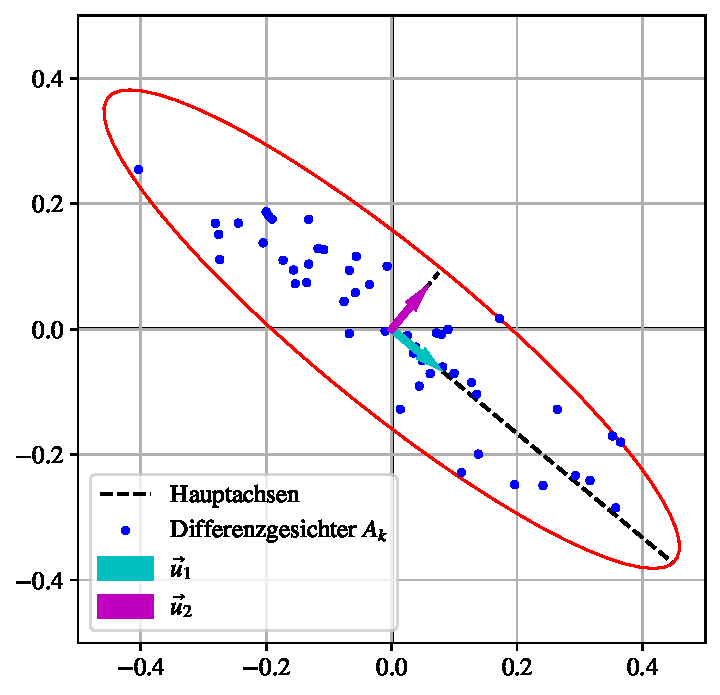
\includegraphics[width=0.45\textwidth]{images/facespace/principal_components} & 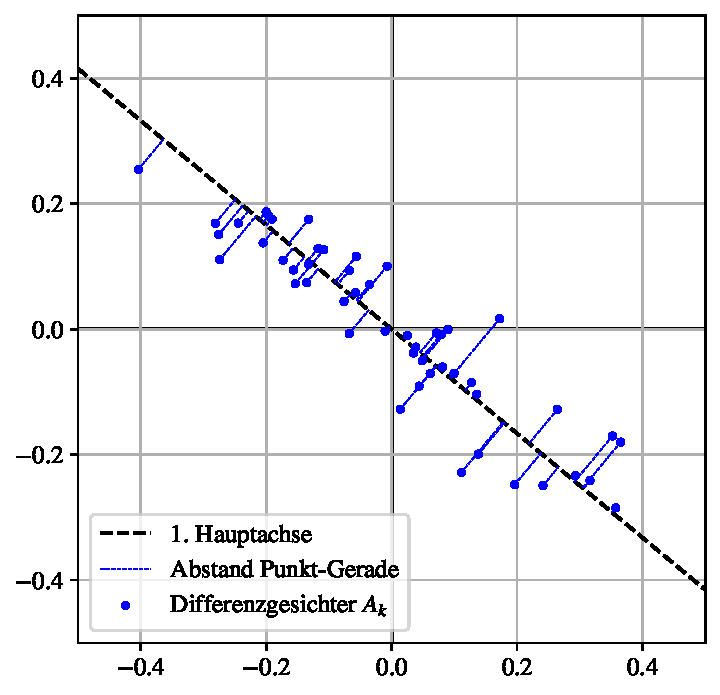
\includegraphics[width=0.45\textwidth]{images/facespace/distance_complicated} \\
	\end{tabular}
	\caption{Die Eigengesichter sind die orthonormalen Vektoren entlang den Hauptachsen.}
	\label{fig:construction}
\end{figure}

Wir werden nun das erste Eigengesicht $\vec{u}_1$ berechnen.
Dazu müssen wir zuerst verstehen was es bedeutet, einen Vektor \glqq{}entlang der grössten Streuung\grqq{} zu finden.
Die erste Hauptachse wird wie folgt bestimmt:
Sie ist diejenige Gerade, welche die Summe der Abstandsquadrate zu den Punkten $A_1,\ldots,A_K$ minimiert.
Dies ist rechts in Abbildung~\ref{fig:construction} gezeigt.
Um die Eigengesichter zu berechnen, müssen wir also den Abstand eines Punktes von einer Geraden berechnen können.
\begin{aufgabe} \label{aufg:distance_simple}
	\phantom{text}\\
	\begin{minipage}{0.55\textwidth}
		Berechnen Sie den Abstand des Punktes $A$ von der Geraden durch Null in Richtung $\vec{u}$, wobei $\vec{a}=\overrightarrow{OA}$ und
		\begin{align*}
			\vec{a}=
			\begin{pmatrix}
				1 \\
				-2
			\end{pmatrix},\quad
			\vec{u}=\frac{1}{5}
			\begin{pmatrix}
				4 \\
				-3
			\end{pmatrix}.
		\end{align*}
		\textit{Hinweis}: Der Vektor $\vec{u}$ hat Länge~1.
	\end{minipage}\hfill
	\begin{minipage}{0.4\textwidth}
		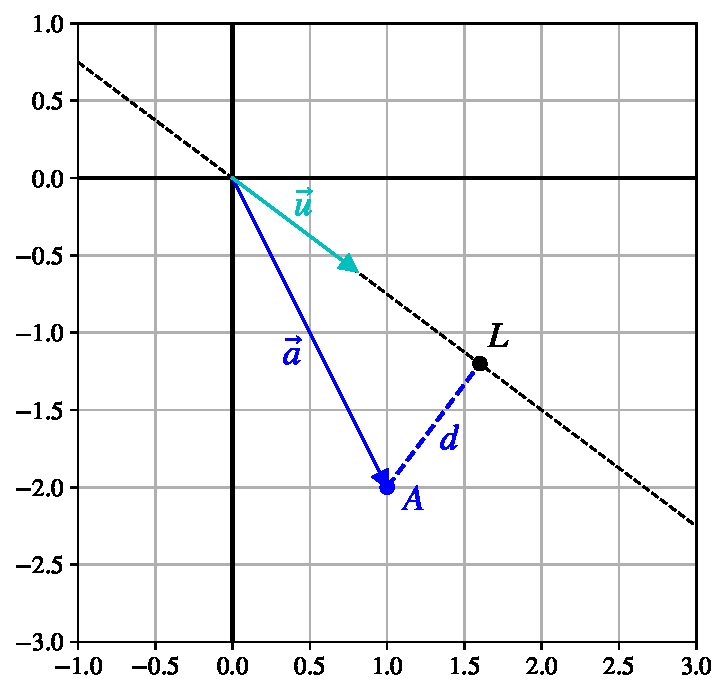
\includegraphics[width=\textwidth]{images/facespace/distance_simple}
	\end{minipage}
\end{aufgabe}
\begin{losung}
	Der Lotfusspunkt $L$ bezeichnet den Punkt auf der Geraden, welcher $A$ am nächsten liegt.
	Der Abstand von $L$ zum Ursprung ist $\vec{a}\cdot\vec{u}=2$.
	Dabei haben wir verwendet, dass $\vec{u}$ Länge 1 hat.
	Die gesuchte Distanz (blaue gestrichelte Linie im Bild) bezeichnen wir mit $d$.
	Nach dem Satz von Pythagoras gilt dann
	\begin{equation*}
		d^2+\left(\vec{a}\cdot\vec{u}\right)^2=\lVert\vec{a}\rVert^2.
	\end{equation*}
	Durch umformen erhalten wir
	\begin{equation*}
		d^2=\lVert\vec{a}\rVert^2-\left(\vec{a}\cdot\vec{u}\right)^2=5-4=1.
	\end{equation*}
	Der Abstand von $A$ zu Geraden ist also $d=1$.
\end{losung}
Was wir in Aufgabe~\ref{aufg:distance_simple} berechnet haben, funktioniert auch in höheren Dimensionen.
Seien $\vec v,\vec w\in\mathbb R^n$, wobei möglicherweise $n>3$.
Das Skalarprodukt dieser Vektoren ist dann definiert als
\begin{equation*}
	\vec v\cdot\vec w=v_1w_1+\ldots+v_nw_n.
\end{equation*}
Ganz analog ist auch das Quadrat Länge eines Vektors gegeben durch $\lVert\vec v\rVert^2=\vec v\cdot\vec v$.
Der Abstand eines Punktes zu einer Geraden berechnet sich dann nach der selben Formel wie in der Lösung von Aufgabe~\ref{aufg:distance_simple}.
\begin{aufgabe} \label{aufg:distance_complex}
	Sei $\vec{u}\in\mathbb R^{M\cdot N}$ ein Vektor der Länge~1.
	Dieser definiert die Gerade durch Null in Richtung $\vec{u}$.
	Finden Sie eine Formel für die Summe der Abstandsquadrate aller Differenzgesichter $A_1,\ldots,A_K$ zu dieser Geraden.
	Dies ist rechts in Abbildung~\ref{fig:construction} dargestellt.
\end{aufgabe}
\begin{losung}
	Wir konzentrieren uns zuerst auf ein beliebiges Differenzgesicht $\vec{a}_k=\overrightarrow{OA_k}$, wobei $1\leq k\leq K$.
	Dessen Abstand zur Geraden bezeichnen wir mit $d_k$.
	Analog zu Aufgabe~\ref{aufg:distance_simple} gilt
	\begin{equation*}
		d_k^2=\lVert\vec{a}_k\rVert^2-\left(\vec{a}_k\cdot\vec{u}\right)^2.
	\end{equation*}
	Die Summe dieser Abstandsquadrate $d_1^2+\ldots+d_K^2$ ist demnach gegeben durch
	\begin{equation*}
		\lVert\vec{a}_1\rVert^2-\left(\vec{a}_1\cdot\vec{u}\right)^2
		+\lVert\vec{a}_2\rVert^2-\left(\vec{a}_2\cdot\vec{u}\right)^2
		+\ldots+
		\lVert\vec{a}_{M\cdot N}\rVert^2-\left(\vec{a}_{M\cdot N}\cdot\vec{u}\right)^2.
	\end{equation*}
\end{losung}
Die Formel aus Aufgabe~\ref{aufg:distance_complex} liefert für jedes $\vec{u}$ einen positiven Wert.
Dasjenige $\vec{u}$, welches diesen Ausdruck minimiert, ist das erste Eigengesicht $\vec{u}_1$.
Die Eigengesichter zu berechnen, heisst also ein Minimierungsproblem zu lösen.
Dies ist nicht so einfach und ist daher bereits implementiert.

Die Eigengesichter wollen wir nun visualisieren, indem wir sie wieder als Bilder darstellen.
Doch da gibt es noch ein Problem.
Die Komponenten der Eigengesichter liegen nicht notwendigerweise in $\left[0,1\right]$ und können daher nicht als Graustufen interpretiert werden.
Damit man sie als Bilder darstellen kann, müssen wir deren Komponenten zuerst wie folgt nach $\left[0,1\right]$ abbilden.
Sei $\vec v\in\mathbb R^{M\cdot N}$ irgend ein Vektor, dessen Komponenten nicht notwendigerweise in $\left[0,1\right]$ liegen.
Sei $\min\left(\vec v\right)$ das Minimum und $\max\left(\vec v\right)$ das Maximum aller Komponenten von $\vec v$.
Wir betrachten nun den Vektor
\begin{equation*}
	\vec w=
	\begin{pmatrix}
		w_1 \\
		w_2 \\
		\vdots \\
		w_{M\cdot N}
	\end{pmatrix}
\end{equation*}
dessen Komponenten sich aus denen von $\vec v$ wie folgt zusammensetzen
\begin{equation*}
	w_i=\frac{v_i-\min\left(\vec v\right)}{\max\left(\vec v\right)-\min\left(\vec v\right)},
\end{equation*}
für alle $i\in\left\{1,\ldots,M\cdot N\right\}$.
Die Komponenten des Vektors $\vec w$ liegen dann alle in $\left[0,1\right]$.
Falls alle Komponenten von $\vec v$ gleich sind, ist $\min\left(\vec v\right)=\max\left(\vec v\right)$ und wir haben eine Division durch Null.
Wir ignorieren diesen Fall.
\begin{aufgabe} \label{aufg:scaling_theory}
	\phantom{text}
	\begin{enumerate}[label=(\alph*)]
		\item Betrachten Sie den Vektor
		\begin{equation*}
			\vec v=
			\begin{pmatrix}
				-2 \\
				4 \\
				1
			\end{pmatrix},
		\end{equation*}
		dessen Komponenten nicht alle in $\left[0,1\right]$ liegen.
		Berechnen Sie daraus den Vektor $\vec w$ gemäss obigem Verfahren.
		\item Begründen Sie, warum dieses Verfahren immer einen Vektor mit Komponenten in $\left[0,1\right]$ liefert, auch für einen allgemeinen Vektor $\vec v$.
	\end{enumerate}
\end{aufgabe}
\begin{losung}
	\phantom{text}
	\begin{enumerate}[label=(\alph*)]
		\item In obigem Beispiel ist $\min\left(\vec v\right)=-2$ und $\max\left(\vec v\right)=4$.
		Daraus ergibt sich für alle $i\in\left\{1,2,3\right\}$
		\begin{equation*}
			w_i=\frac{v_i-\left(-2\right)}{4-\left(-2\right)}=\frac{v_i+2}{6}.
		\end{equation*}
		Somit erhalten wir
		\begin{equation*}
			\vec w=
			\begin{pmatrix}
				0 \\
				1 \\
				\tfrac{1}{2}
			\end{pmatrix}.
		\end{equation*}
		\item Für alle Komponenten $v_i$ gilt stets
		\begin{equation*}
			\min\left(\vec v\right)\leq v_i\leq\max\left(\vec v\right).
		\end{equation*}
		Daraus folgt, dass im Bruch
		\begin{equation*}
			w_i=\frac{v_i-\min\left(\vec v\right)}{\max\left(\vec v\right)-\min\left(\vec v\right)},
		\end{equation*}
		der Nenner immer grösser oder Gleich dem Zähler ist, und dass beide nicht negativ werden können.
		Folglich muss $w_i\in\left[0,1\right]$ gelten.
	\end{enumerate}
\end{losung}
\begin{aufgabe} \label{aufg:scaling_code}
	Ergänzen Sie die Funktion \texttt{interpolate(v)}, welche den Vektor mit Komponenten in $\left[0,1\right]$ zurück gibt, der aus dem Vektor \texttt{v} durch obiges Verfahren entsteht.
	Testen Sie ihre Lösung mit dem Python Skript \texttt{plot\_eigenfaces.py}, welches ihre Funktion \texttt{interpolate(v)} auf die Eigengesichter $\vec u_1,\ldots,\vec u_K$ anwendet und diese als Bilder abspeichert.
	\textit{Hinweis:} Die Funktionen \texttt{np.min(v)} und \texttt{np.max(v)} liefern das Minimum und das Maximum eines Vektors \texttt{v}.
\end{aufgabe}
\begin{losung}
	Eine mögliche Lösung ist unten gezeigt.
	Die Eigengesichter sind in Abbildung~\ref{fig:eigenfaces} dargestellt.
\begin{lstlisting}[style=python]
import numpy as np

def interpolate(v):
	w = np.zeros_like(v)
	a = np.min(v)
	b = np.max(v)
	for vi, wi in zip(v, w):
		wi = (vi - a) / (b - a)
	return w
\end{lstlisting}
\end{losung}

\begin{figure}[ht]
	\centering
	\begin{tabular}{cccccccc}
		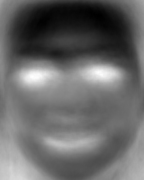
\includegraphics[width=0.1\textwidth]{images/eigenfaces/eigenface00} & 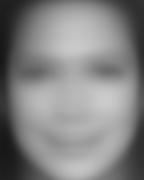
\includegraphics[width=0.1\textwidth]{images/eigenfaces/eigenface01} &
		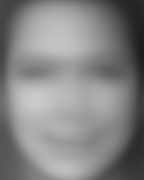
\includegraphics[width=0.1\textwidth]{images/eigenfaces/eigenface02} & 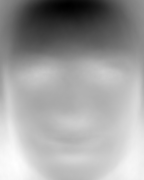
\includegraphics[width=0.1\textwidth]{images/eigenfaces/eigenface03} &
		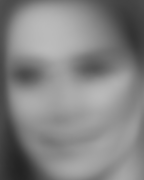
\includegraphics[width=0.1\textwidth]{images/eigenfaces/eigenface04} &
		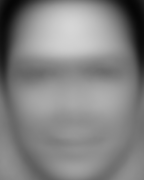
\includegraphics[width=0.1\textwidth]{images/eigenfaces/eigenface05} & 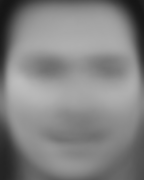
\includegraphics[width=0.1\textwidth]{images/eigenfaces/eigenface06} &
		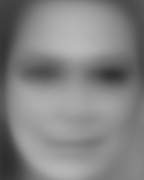
\includegraphics[width=0.1\textwidth]{images/eigenfaces/eigenface07} \\ 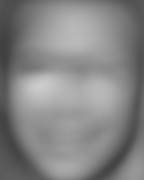
\includegraphics[width=0.1\textwidth]{images/eigenfaces/eigenface08} &
		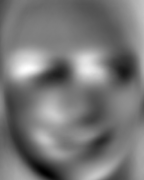
\includegraphics[width=0.1\textwidth]{images/eigenfaces/eigenface09} & 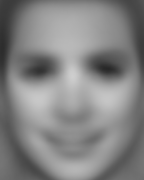
\includegraphics[width=0.1\textwidth]{images/eigenfaces/eigenface10} &
		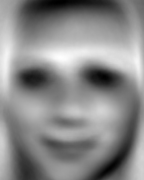
\includegraphics[width=0.1\textwidth]{images/eigenfaces/eigenface11} & 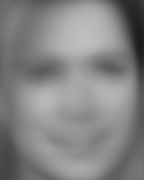
\includegraphics[width=0.1\textwidth]{images/eigenfaces/eigenface12} &
		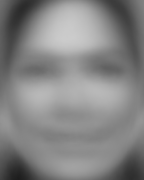
\includegraphics[width=0.1\textwidth]{images/eigenfaces/eigenface13} & 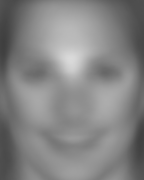
\includegraphics[width=0.1\textwidth]{images/eigenfaces/eigenface14} &
		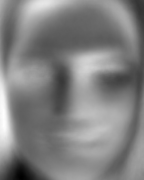
\includegraphics[width=0.1\textwidth]{images/eigenfaces/eigenface15} \\
	\end{tabular}
	\caption{Die ersten 16 Eigengesichter wurden wieder als Bild dargestellt.}
	\label{fig:eigenfaces}
\end{figure}

Im Grunde fangen die Eigengesichter charakteristische Gesichtszüge ein.
Mit charakteristisch ist hier gemeint, dass genau diese Gesichtszüge für die grösste Streuung unter allen Bildern der Datenbank verantwortlich sind.
Sie beschreiben die Merkmale, nach denen sich die Gesichter am meisten unterscheiden.
Besser gesagt: Das erste Eigengesicht fängt den Gesichtszug mit der grössten Streuung ein.
Die weiteren Eigengesichter fangen Gesichtszüge mit immer weniger Streuung ein.
Dies spiegelt sich auch in deren Konstruktion wieder, welche die Eigengesichter ja gerade als Vektoren entlang der grössten Streuung definiert.
\section{Vom Bild zum Vektor} \label{sec:vectormatrix}
\begin{tcolorbox}
	\centerline{\textbf{Lernziele Kapitel~\ref{sec:vectormatrix}}}
	\begin{enumerate}[leftmargin=*,label=\thesection.\arabic*]
		\item \label{item:vectormatrix_theory} Die Lernenden können für niedrige Auflösung ($M\cdot N<10$) die Umrechnungen zwischen Bild, Matrix und Vektor von Hand ausführen.\\
		(Aufgabe~\ref{aufg:vectormatrix_theory} und~\ref{aufg:vectormatrix_theory_1})
		\item \label{item:vectormatrix_code} Die Lernenden können in Python die Einträge von Vektoren und Matrizen auslesen und verändern.\\
		(Aufgabe~\ref{aufg:vectormatrix_code} und~\ref{aufg:negative})
	\end{enumerate}
\end{tcolorbox}
Der erste Schritt besteht darin, Bilder als Vektoren aufzufassen.
Das hat zwei Gründe: Erstens können wir diese nur so geeignet in Python darstellen und manipulieren.
Zweitens erlaubt uns das, Bilder in den Kontext der linearen Algebra zu bringen um deren mächtige Methoden anzuwenden.
Als Beispiel betrachten wir ein Bild der Auflösung $M=180$ Pixel (Höhe) mal $N=144$ Pixel (Breite), wie in Abbildung~\ref{fig:image_to_vector}.
Jedem Pixel wird nun eine reelle Zahl zwischen 0 und 1 zugeordnet.
Dabei bedeutet 0, dass das Pixel schwarz ist und 1 bedeutet, dass es weiss ist.
Die reellen Zahlen dazwischen beschreiben die Graustufen.
Wir Nummerieren diese Pixel mit zwei Indices $\left(m,n\right)$, wobei $1\leq m\leq M$ und $1\leq n\leq N$.
Zum Beispiel entspricht $\left(1,N\right)$ dem Pixel in der oberen rechten Ecke des Bildes.
Diesem Pixel wird also eine Zahl $p_{mn}$ zugeordnet, wobei $0\leq p_{mn}\leq 1$.
Das gibt uns eine $M\times N$-Matrix deren Einträge gerade die $p_{mn}$ sind.
So können wir also ein schwarz-weiss Bild als Matrix auffassen.
Nun schreiben wir die Spalten dieser Matrix in einen Vektor wie in Abbildung~\ref{fig:image_to_vector} gezeigt.
Damit erhalten wir eine eindeutige Korrespondenz zwischen schwarz-weiss Bilder der Auflösung $M\times N$ und Vektoren der Länge $M\cdot N$ mit Einträgen zwischen 0 und 1.
Für diesen Schritt ist es egal ob das Bild ein Gesicht zeigt oder etwas anderes.
\begin{figure}[ht]
	\centering
	\begin{tabular}{m{3.5cm} m{1cm} c m{1cm} c}
		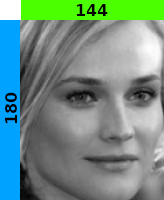
\includegraphics[width=0.2\textwidth]{images/vectormatrix/ImageToVector} &
		$\longleftrightarrow$ &
		$\begin{pmatrix}
			\textcolor{violet}{p_{11}} & \textcolor{orange}{p_{12}} & \cdots & \textcolor{olive}{p_{1N}} \\
			\textcolor{violet}{\vdots} & \textcolor{orange}{\vdots} & \ddots & \textcolor{olive}{\vdots} \\
			\textcolor{violet}{p_{M1}} & \textcolor{orange}{p_{M2}} & \cdots &  \textcolor{olive}{p_{MN}} \\
		\end{pmatrix}$ &
		$\longleftrightarrow$ &
		$\begin{pmatrix}
			\textcolor{violet}{p_{11}} \\
			\textcolor{violet}{\vdots} \\
			\textcolor{violet}{p_{M1}} \\
			\textcolor{orange}{p_{12}} \\
			\textcolor{orange}{\vdots} \\
			\textcolor{orange}{p_{M2}} \\
			\vdots \\
			\textcolor{olive}{p_{1N}} \\
			\textcolor{olive}{\vdots} \\
			\textcolor{olive}{p_{MN}} \\
		\end{pmatrix}$
	\end{tabular}
	\caption{Ein schwarz-weiss Bild kann als Matrix oder Vektor aufgefasst werden.}
	\label{fig:image_to_vector}
\end{figure}
\pagebreak[4]
\begin{aufgabe} \label{aufg:vectormatrix_theory}
	Man betrachte das schwarz-weiss Bild, welches durch folgende Matrix beschrieben ist.
	\begin{equation*}
		\begin{pmatrix}
			1 & \frac{1}{4} \\
			\frac{1}{2} & 0 \\
			0 & \frac{3}{4} \\
		\end{pmatrix}
	\end{equation*}
	\begin{enumerate}[label=(\alph*)]
		\item Welche Werte für $M$ und $N$ beschreiben die Auflösung dieses Bildes?
		\item Wie sieht der Vektor aus, der dieses Bild beschreibt?
		\item \label{item:image3x2} Welches der folgenden drei Bilder entspricht dieser Matrix?
		
		\definecolor{onefourth}{rgb}{0.25, 0.25, 0.25}
		\definecolor{onehalf}{rgb}{0.5, 0.5, 0.5}
		\definecolor{threefourth}{rgb}{0.75, 0.75, 0.75}
		
		\qquad\qquad
		\begin{tikzpicture}
			\draw[step=1cm,white,very thin] (0,0) grid (2,3);
			\fill[white] (0,0) rectangle (1,1);
			\fill[onefourth] (1,0) rectangle (2,1);
			\fill[onehalf] (0,1) rectangle (1,2);
			\fill[white] (1,1) rectangle (2,2);
			\fill[black] (0,2) rectangle (1,3);
			\fill[threefourth] (1,2) rectangle (2,3);
		\end{tikzpicture}
		\qquad\qquad
		\begin{tikzpicture}
			\draw[step=1cm,white,very thin] (0,0) grid (2,3);
			\fill[black] (0,0) rectangle (1,1);
			\fill[threefourth] (1,0) rectangle (2,1);
			\fill[onehalf] (0,1) rectangle (1,2);
			\fill[black] (1,1) rectangle (2,2);
			\fill[white] (0,2) rectangle (1,3);
			\fill[onefourth] (1,2) rectangle (2,3);
		\end{tikzpicture}
		\qquad\qquad
		\begin{tikzpicture}
			\draw[step=1cm,white,very thin] (0,0) grid (2,3);
			\fill[black] (0,0) rectangle (1,1);
			\fill[onefourth] (1,0) rectangle (2,1);
			\fill[onehalf] (0,1) rectangle (1,2);
			\fill[black] (1,1) rectangle (2,2);
			\fill[white] (0,2) rectangle (1,3);
			\fill[threefourth] (1,2) rectangle (2,3);
		\end{tikzpicture}
	\end{enumerate}
\end{aufgabe}
\begin{losung}
	Die Lösung der ersten beiden Teilaufgaben kann von Abbildung~\ref{fig:image_to_vector} abgelesen werden.
	Für die letzte Teilaufgabe erinnern wir uns, dass die Zahlen zwischen 0 und 1 fliessend den Graustufen von Schwarz (Null) bis Weiss (Eins) entsprechen.
	\begin{enumerate}[label=(\alph*)]
		\item Die Auflösung ist $M=3$ mal $N=2$ Pixel.
		\item Der Vektor ist gegeben durch
		\begin{equation*}
			\begin{pmatrix}
				1 \\ \frac{1}{2} \\ 0 \\ \frac{1}{4} \\ 0 \\ \frac{3}{4} \\
			\end{pmatrix}.
		\end{equation*}
		\item Das mittlere Bild entspricht der Matrix.
	\end{enumerate}
\end{losung}
\begin{aufgabe} \label{aufg:vectormatrix_theory_1}
	Man betrachte den Vektor
	\begin{equation*}
		\begin{pmatrix}
			\frac{3}{4} \\ 0 \\ \frac{1}{4} \\ 0 \\ \frac{1}{2} \\ 1
		\end{pmatrix}.
	\end{equation*}
	Dieser soll ein Bild der Auflösung $M=2$ und $N=3$ beschreiben.
	\begin{enumerate}[label=(\alph*)]
		\item Schreiben Sie die entsprechende Matrix gemäss Abbildung~\ref{fig:image_to_vector} auf.
		\item Zeichnen Sie das entsprechende schwarz-weiss Bild, analog zu Teil~\ref{item:image3x2} in Aufgabe~\ref{aufg:vectormatrix_theory}.
	\end{enumerate}
\end{aufgabe}
\begin{losung}
	\begin{enumerate}[label=(\alph*)]
		\item Die Matrix hat nun $M=2$ Zeilen und $N=3$ Spalten. Nach Abbildung~\ref{fig:image_to_vector} erhalten wir
		\begin{equation*}
			\begin{pmatrix}
				\frac{3}{4} & 0 & \frac{1}{4} \\
				0 & \frac{1}{2} & 1
			\end{pmatrix}.
		\end{equation*}
		\item Das entsprechende schwarz-weiss Bild lässt sich von obiger Matrix ablesen:
		
		\definecolor{onefourth}{rgb}{0.25, 0.25, 0.25}
		\definecolor{onehalf}{rgb}{0.5, 0.5, 0.5}
		\definecolor{threefourth}{rgb}{0.75, 0.75, 0.75}
		\begin{center}
		\begin{tikzpicture}
			\draw[step=1cm,white,very thin] (0,0) grid (3,2);
			\fill[white] (0,0) rectangle (1,1);
			\fill[onehalf] (1,0) rectangle (2,1);
			\fill[black] (2,0) rectangle (3,1);
			\fill[onefourth] (0,1) rectangle (1,2);
			\fill[white] (1,1) rectangle (2,2);
			\fill[threefourth] (2,1) rectangle (3,2);
		\end{tikzpicture}
		\end{center}

		Natürlich können Sie nicht die exakten Graustufen wiedergeben.
		Aber ihr Bild sollte vier verschiedene Graustufen enthalten, die richtig auf die Pixel verteilt sind.
	\end{enumerate}
\end{losung}
In unserem Python Code ist die Funktion, welche eine $M\times N$ Matrix auf diese Weise in einen Vektor der Länge $M\cdot N$ überführt, bereits implementiert.
Sie befindet sich im File \texttt{eigenfaces.py} und heisst \texttt{matrix\_to\_vector}.
Wir betrachten diese nun etwas genauer, um die Manipulation von Matrizen und Vektoren in Python zu lernen.
\begin{lstlisting}[style=python]
import numpy as np

def matrix_to_vector(P, M, N):
	v = np.zeros(M * N)
	for m in range(M):
		for n in range(N):
			v[n + N * m] = P[m, n]
	return v
\end{lstlisting}
Das Argument \texttt{P} ist eine \texttt{M} mal \texttt{N} Matrix und besteht aus den Einträgen $p_{mn}$ wie oben.
Auf die Einträge von Vektoren und Matrizen kann über die eckigen Klammern $[\ldots]$ zugegriffen werden.
Wir brauchen aber auch die Umkehrung dieser Operation.
Das ist der Zweck folgender Übung.
\begin{aufgabe} \label{aufg:vectormatrix_code}
	Ergänzen Sie im File \texttt{eigenfaces.py} die Funktion \texttt{vector\_to\_matrix(v, M, N)}.
	Dabei ist \texttt{v} ein Vektor der Länge $\texttt{M}\cdot\texttt{N}$ wie oben.
	Die Funktion soll die zu \texttt{v} gehörende Matrix zurück geben.
	Sie können die ihre Lösung überprüfen indem Sie das Skript \texttt{vector\_to\_matrix\_test.py} laufen lassen.
\end{aufgabe}
\begin{losung}
	Bei einer richtigen Lösung sollte das Skript \texttt{vector\_to\_matrix\_test.py} das Foto aus Abbildung~\ref{fig:image_to_vector} generieren.
	Die Lösung könnte zum Beispiel so aussehen:
\begin{lstlisting}[style=python]
import numpy as np

def vector_to_matrix(v, M, N):
	P = np.zeros((M, N))
	for m in range(M):
		for n in range(N):
			P[m, n] = v[n + N * m]
	return P
\end{lstlisting}
\end{losung}
Man kann gewisse Effekte in einem Bild erzeugen, indem man den zugehörigen Vektor manipuliert und anschliessend wieder als Bild darstellt.
Zum Beispiel kann man das Negativ eines gegebenen schwarz-weiss Bildes generieren.
Dazu nimmt man den Vektor $\vec p$ der Länge $M\cdot N$, welcher dieses Bild darstellt, und definiert damit einen neuen Vektor wie folgt
\begin{equation*}
	\vec p=
	\begin{pmatrix}
		p_1 \\ p_2 \\ \vdots \\ p_{M\cdot N} \\
	\end{pmatrix}
	\quad\longrightarrow\quad
	\begin{pmatrix}
		1-p_1 \\ 1-p_2 \\ \vdots \\ 1-p_{M\cdot N} \\
	\end{pmatrix}.
\end{equation*}
Der Vektor auf der rechten Seite entspricht dem Negativ des ursprünglichen Bildes.
Wie dieses Bild genau aussieht, sehen wir in der nächsten Aufgabe.
\begin{aufgabe} \label{aufg:negative}
	Ergänzen Sie im Skript \texttt{negative.py} die Funktion \texttt{get\_negative.py}.
	Diese soll zu einem gegeben Vektor \texttt{p} mit Einträgen zwischen 0 und 1 den Vektor des entsprechenden Negativs zurückgeben, wie oben beschrieben.
	Lassen Sie das Skript \texttt{negative.py} laufen um das entsprechende Bild auszugeben und um Ihre Lösung zu überprüfen.
\end{aufgabe}
\begin{losung}
	Links ist eine mögliche Implementierung gezeigt.
	Rechts ist ein Bild und dessen Negativ.\\[0.5cm]
	\begin{minipage}{0.45\textwidth}
\begin{lstlisting}[style=python]
def get_negative(p):
	MN = len(p)
	for i in range(MN):
		p[i] = 1.0 - p[i]
	return p
\end{lstlisting}
	\end{minipage}\hfill
	\begin{minipage}{0.25\textwidth}\vspace{-1cm}
		\centering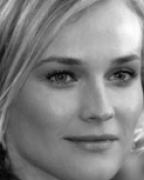
\includegraphics[width=0.6\textwidth]{images/vectormatrix/Diane_Kruger}
	\end{minipage}
	\begin{minipage}{0.25\textwidth}\vspace{-1cm}
		\centering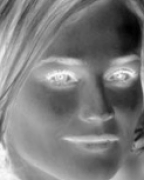
\includegraphics[width=0.6\textwidth]{images/vectormatrix/Diane_Kruger_negative}
	\end{minipage}
\end{losung}
\section{Durchschnittsgesicht und Differenzgesichter} \label{sec:facespace}
\begin{tcolorbox}
	\centerline{\textbf{Lernziele Kapitel~\ref{sec:facespace}}}
	\begin{enumerate}[leftmargin=*,label=\thesection.\arabic*]
		\item \label{item:meandiff_simple} Die Lernenden können den Durchschnitt einer Familie von Vektoren von Hand berechnen (für konkrete Zahlenbeispiele).\\
		(Aufgaben~\ref{aufg:meandiff_simple} und~\ref{aufg:meandiff_simple_1})
		\item \label{item:meanface} Die Lernenden können die Addition und Subtraktion von Vektoren und deren Multiplikation mit einem Skalar in Python ausführen.\\
		(Aufgaben~\ref{aufg:meanface} und~\ref{aufg:diffface})
		\item \label{item:hmmc} Die Lernenden können die Begriffe Durchschnittsgesicht und Differenzgesicht erklären.\\
		(Aufgaben~\ref{aufg:difffaces_images} und~\ref{aufg:hmmc})
	\end{enumerate}
\end{tcolorbox}
Wir haben im letzten Kapitel gesehen, dass man Bilder der Auflösung $M\times N$ als Vektoren der Länge $M\cdot N$ auffassen kann.
Diese Vektoren können wir wiederum als Punkte in einem Raum der Dimension $M\cdot N$ auffassen.
In diesem Kapitel werden wir diese Sichtweise ausarbeiten.

Sei $K$ die Anzahl aller Bilder unserer Datenbank.
Jedes Bild soll dabei die Auflösung $M\times N$ haben.
Weiter seien $\vec b_1,\ldots,\vec b_K$ die Vektoren dieser Bilder.
Diese Darstellung erlaubt uns, das \textit{Durchschnittsgesicht}, wir nennen es $\vec m$, zu definieren
\begin{equation*}
	\vec m=\frac{1}{K}\left(\vec b_1+\ldots+\vec b_K\right).
\end{equation*}
Dies ist einfach die Summe der Vektoren dividiert durch deren Anzahl.
Wegen dieser Analogie zum arithmetischen Mittel, nennen wir dies das Durchschnittsgesicht.
Damit können wir die sogenannten \textit{Differenzgesichter} $\vec a_1,\ldots,\vec a_K$ bilden.
Diese sind definiert als als die Verschiebung der Gesichter aus der Datenbank um $-\vec{m}$, also
\begin{equation*}
	\vec a_k=\vec b_k-\vec m,\quad k=1,\ldots,K.
\end{equation*}
Um den Durchschnitt und die Verschiebung von Vektoren geometrisch besser zu verstehen, schauen wir das zuerst in der Ebene an.
\begin{aufgabe} \label{aufg:meandiff_simple}
	Betrachten Sie die folgenden drei Vektoren
	\begin{equation*}
		\vec{b}_1=
		\begin{pmatrix}
			-4 \\
			-5
		\end{pmatrix},\quad
		\vec{b}_2=
		\begin{pmatrix}
			9 \\
			-5
		\end{pmatrix},\quad
		\vec{b}_3=
		\begin{pmatrix}
			1 \\
			7
		\end{pmatrix}.
	\end{equation*}
	\begin{enumerate}[label=(\alph*)]
		\item Berechnen Sie den Durchschnitt $\vec{m}$ der Vektoren $\vec{b}_1,\vec{b}_2,\vec{b}_3$.
		\item \label{item:difference_faces} Berechnen Sie die um $-\vec{m}$ verschobenen Vektoren
		\begin{equation*}
			\vec{a}_1=\vec{b}_1-\vec{m},\quad
			\vec{a}_2=\vec{b}_2-\vec{m},\quad
			\vec{a}_3=\vec{b}_3-\vec{m}.
		\end{equation*}
		\item Zeichnen Sie alle Vektoren $\vec{a}_1,\vec{a}_2,\vec{a}_3$ und $\vec{b}_1,\vec{b}_2,\vec{b}_3$, sowie $\vec{m}$ in ein Koordinatensystem.
	\end{enumerate}
\end{aufgabe}
\begin{losung}
	\begin{enumerate}[label=(\alph*)]
		\item Wie im skalaren Fall ist der Durchschnitt definiert als die Summe geteilt durch dir Anzahl der Summanden, also
		\begin{equation*}
			\vec{m}=\frac{1}{3}\left(\vec{b}_1+\vec{b}_2+\vec{b}_3\right)
			=\frac{1}{3}\left(
			\begin{pmatrix}
				-4 \\
				-5
			\end{pmatrix}+
			\begin{pmatrix}
				9 \\
				-5
			\end{pmatrix}+
			\begin{pmatrix}
				1 \\
				7
			\end{pmatrix}
			\right)
			=
			\begin{pmatrix}
				2 \\
				-1
			\end{pmatrix}.
		\end{equation*}
		\item Für die um $-\vec{m}$ verschobenen Vektoren erhalten wir folglich
		\begin{equation*}
			\vec{a}_1=
			\begin{pmatrix}
				-6 \\
				-4
			\end{pmatrix},\quad
			\vec{a}_2=
			\begin{pmatrix}
				7 \\
				-4
			\end{pmatrix},\quad
			\vec{a}_3=
			\begin{pmatrix}
				-1 \\
				8
			\end{pmatrix}.
		\end{equation*}
		\item Die Skizze ist in Abbildung~\ref{fig:meanddiff_simple} dargestellt.
			Gezeichnet sind die Vektoren aufgefasst als Punkte, also
			\begin{equation*}
				\vec{m}=\overrightarrow{OM},\qquad
				\vec{a}_k=\overrightarrow{OA_k},\qquad
				\vec{b}_k=\overrightarrow{OB_k},\qquad
				k=1,2,3.
			\end{equation*}
			\begin{center}
			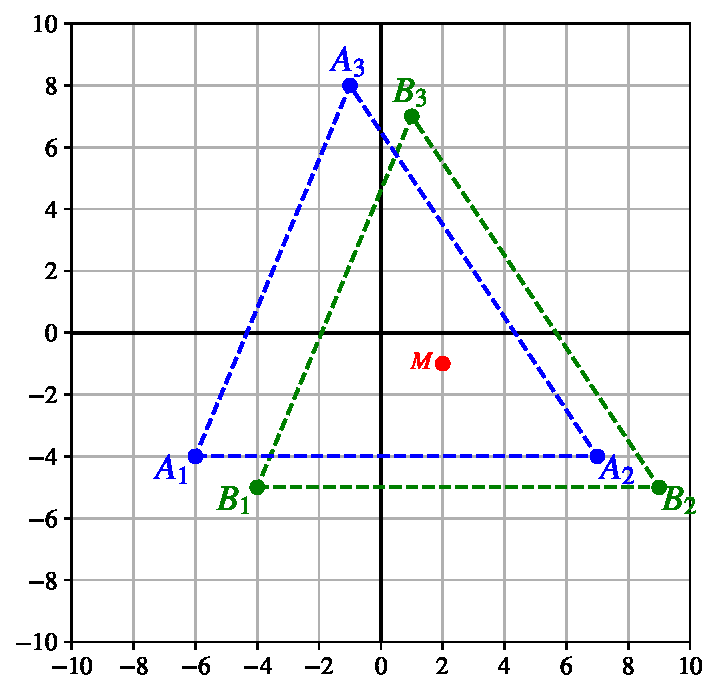
\includegraphics[width=0.5\textwidth]{images/facespace/meandiff_simple}
			\captionof{figure}{Durchschnitt $\vec{m}$ der Vektoren $\vec{b}_1,\vec{b}_2,\vec{b}_3$ sowie deren Translationen $\vec{a}_1,\vec{a}_2,\vec{a}_3$ um $-\vec{m}$, alle aufgefasst als Punkte in der Ebene.}
			\label{fig:meanddiff_simple}
			\end{center}
	\end{enumerate}
\end{losung}
\begin{aufgabe} \label{aufg:meandiff_simple_1}
	Betrachten Sie die Vektoren
	\begin{equation*}
		\vec{b}_1=
		\begin{pmatrix}
			-2 \\
			-1 \\
			1
		\end{pmatrix},\qquad
		\vec{b}_2=
		\begin{pmatrix}
			4 \\
			-1 \\
			1
		\end{pmatrix}.
	\end{equation*}
	\begin{enumerate}[label=(\alph*)]
		\item Berechnen Sie den Durchschnitt $\vec{m}$ der Vektoren $\vec{b}_1$ und $\vec{b}_2$.
		\item Berechnen Sie die um $-\vec{m}$ verschobenen Vektoren
		\begin{equation*}
			\vec{a}_1=\vec{b}_1-\vec{m}
			\qquad\text{und}\qquad
			\vec{a}_2=\vec{b}_2-\vec{m}.
		\end{equation*}
		\item Was ist der Durchschnitt der Vektoren $\vec a_1$ und $\vec a_2$? Was ist der Durchschnitt der Vektoren $\vec a_1,\vec a_2,\vec a_3$ aus Teilaufgabe~\ref{aufg:meandiff_simple}~\ref{item:difference_faces}?
	\end{enumerate}
\end{aufgabe}
\begin{losung}
	\begin{enumerate}[label=(\alph*)]
		\item Wir berechnen die Summe der beiden Vektoren und dividieren durch deren Anzahl
		\begin{equation*}
			\vec{m}=\frac{1}{2}\left(\vec{b}_1+\vec{b}_2\right)
			=\frac{1}{2}\left(
			\begin{pmatrix}
				-2 \\
				-1 \\
				1
			\end{pmatrix}+
			\begin{pmatrix}
				4 \\
				-1 \\
				1
			\end{pmatrix}
			\right)
			=
			\begin{pmatrix}
				1 \\
				-1 \\
				1
			\end{pmatrix}.
		\end{equation*}
		\item Für die um $-\vec{m}$ verschobenen Vektoren erhalten wir folglich
		\begin{equation*}
			\vec{a}_1=
			\begin{pmatrix}
				-3 \\
				0 \\
				0
			\end{pmatrix},\qquad
			\vec{a}_2=
			\begin{pmatrix}
				3 \\
				0 \\
				0
			\end{pmatrix}.
		\end{equation*}
		\item Der Durchschnitt der verschobenen Vektoren ist
		\begin{equation*}
			\frac{1}{2}\left(\vec{a}_1+\vec{a}_2\right)=
			\frac{1}{2}\left(\begin{pmatrix}
				-3 \\
				0 \\
				0
			\end{pmatrix}+
			\begin{pmatrix}
				3 \\
				0 \\
				0
			\end{pmatrix}\right)=
			\begin{pmatrix}
				0 \\
				0 \\
				0
			\end{pmatrix}.
		\end{equation*}
		Wenn man eine Familie von Vektoren um ihren Durchschnitt verschiebt, erhält haben die resultierenden Vektoren immer den Nullvektor als Durchschnitt.
		Folglicht gilt das auch für die Vektoren aus Teilaufgabe~\ref{aufg:meandiff_simple}~\ref{item:difference_faces}.
	\end{enumerate}
\end{losung}
Nun wollen wir das Durchschnittsgesicht
\begin{equation*}
	\vec m=\frac{1}{K}\left(\vec b_1+\ldots+\vec b_K\right)
\end{equation*}
der Bilder aus der Datenbank berechnen und wieder als Bild ausgeben.
Wie sieht so ein Durchschnittsgesicht aus?
Das werden wir in folgender Übung herausfinden.
\begin{aufgabe} \label{aufg:meanface}
	Ergänzen Sie im File \texttt{eigenfaces.py} die Funktion \texttt{meanface(b\_list)}.
	Dabei ist \texttt{b\_list} die Liste der Länge $K$ der Vektoren $\vec b_1,\ldots,\vec b_K$.
	Der Rückgabewert soll das Durchschnittsgesicht $\vec m$ sein.
	Sie können die ihre Lösung überprüfen indem Sie das Skript \texttt{meanface\_test.py} laufen lassen.
	\textit{Hinweis:} Die Python Funktionen \texttt{len(...) und sum(...)} können nützlich sein.
\end{aufgabe}
\begin{losung}
	Hier ist eine mögliche Lösung und das davon mit \texttt{meanface\_test.py} generierte Durchschnittsgesicht.\\[0.5cm]
	\begin{minipage}{0.45\textwidth}
\begin{lstlisting}[style=python]
def meanface(b_list):
	K = len(b_list)
	return sum(b_list) / K
\end{lstlisting}
	\end{minipage}\hfill
	\begin{minipage}{0.3\textwidth}\vspace{-1cm}
		\centering\hfill Durchschnittsgesicht:
	\end{minipage}
	\begin{minipage}{0.2\textwidth}\vspace{-1cm}
		\centering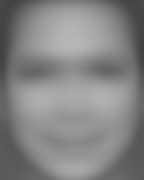
\includegraphics[width=0.6\textwidth]{images/facespace/meanface}
	\end{minipage}
\end{losung}
Nun berechnen wir die \textit{Differenzgesichter} $\vec a_1,\ldots,\vec a_K$, also die Gesichter der Datenbank, welche um $-\vec{m}$ verschoben wurden
\begin{equation*}
	\vec a_k=\vec b_k-\vec m,\quad k=1,\ldots,K.
\end{equation*}
Diese berechnen wir nun in Python.
\begin{aufgabe} \label{aufg:diffface}
	Ergänzen Sie im File \texttt{eigenfaces.py} die Funktion \texttt{diffface(b\_list)}.
	Dabei ist \texttt{b\_list} die Liste der Länge $K$ der Vektoren $\vec b_1,\ldots,\vec b_K$.
	Der Rückgabewert soll eine Liste der Länge $K$ sein, welche die Differenzgesichter $\vec a_1,\ldots,\vec a_K$ gemäss obiger Formel enthält.
	Sie können die ihre Lösung überprüfen indem Sie das Skript \texttt{diffface\_test.py} laufen lassen.
	\textit{Hinweis:} Verwenden Sie die Funktion \texttt{meanface(...)} aus der vorherigen Aufgabe.
\end{aufgabe}
\begin{losung}
	Eine korrekte Lösung könnte so aussehen.
\begin{lstlisting}[style=python]
def diffface(b_list):
	a_list = copy.deepcopy(b_list)
	m = meanface(b_list)
	for k in len(b_list):
		a_list[k] = b_list[k] - m
	return a_list
\end{lstlisting}
\end{losung}
Die eben eingeführten Begriffe sind in Abbildung~\ref{fig:meandiff} für Vektoren mit zwei Komponenten visualisiert.
Die Quintessenz ist, dass sich diese Vektoren (und damit die Bilder) als Punkte in einem Raum der Dimension $M\cdot N$ auffassen lassen.
Wir bezeichnen diese Punkte mit Grossbuchstaben, also ($O$ bezeichnet hier den Ursprung)
\begin{equation*}
	\vec{m}=\overrightarrow{OM},\qquad
	\vec{a}_k=\overrightarrow{OA_k},\qquad
	\vec{b}_k=\overrightarrow{OB_k},\qquad
	k=1,\ldots,K.
\end{equation*}
Die Bilder der Datenbank bilden dann eine \glqq{}Punktewolke\grqq{} in diesem Raum.
Durch Subtraktion von $\vec m$ wir diese Punktewolke um den Ursprung zentriert.
Das Resultat dieser Subtraktion (oder Verschiebung) sind die Differenzgesichter.
Das ist in Abbildung~\ref{fig:meandiff} gezeigt.
\begin{figure}[ht]
	\centering
	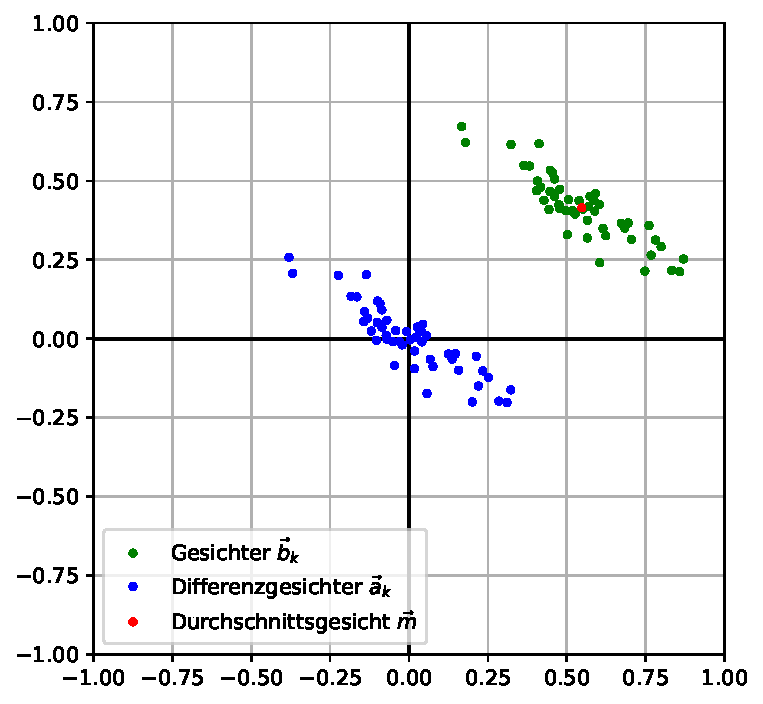
\includegraphics[width=0.5\textwidth]{images/facespace/meandiff}
	\caption{Die Gesichter werden um den Ursprung zentriert indem man das Durchschnittsgesicht subtrahiert.}
	\label{fig:meandiff}
\end{figure}
\begin{aufgabe} \label{aufg:difffaces_images}
	Wir haben in Aufgabe~\ref{aufg:meanface} das Durchschnittsgesicht wieder als Bild dargestellt.
	Könnte man das auch mit den Differenzgesichtern machen?
	Begründen Sie.
\end{aufgabe}
\begin{losung}
	Nein, die Differenzgesichter lassen sich nicht wieder als Bilder darstellen, weil die Einträge dieser Vektoren nicht zwischen 0 und 1 liegen.
	Dies sieht man zum Beispiel in Abbildung~\ref{fig:meandiff}.
	Man kann also diesen Vektor-Einträgen keine Graustufe zuordnen.
\end{losung}
\begin{aufgabe} \label{aufg:hmmc}
	Nennen Sie einen Unterschied und eine Gemeinsamkeit der vereinfachten Darstellung in Abbildung~\ref{fig:meandiff} zu unserer tatsächlichen Situation mit Bildern von Gesichtern.
	Gehen Sie davon aus, dass unsere Bilder eine Auflösung von $M=180$ und $N=144$ haben, wie im letzten Kapitel.
\end{aufgabe}
\begin{losung}
	Als Vektoren aufgefasst sind die Gesichter Punkte im $\mathbb R^{M\cdot N}$.
	Für $M=180$ und $N=144$ wären das Punkte im $\mathbb R^{25'920}$ und nicht im $\mathbb R^2$ wie in der Abbildung.
	Anders ausgedrückt zeigt die Abbildung den Spezialfall $M\cdot N=2$.
	Das entspricht Bilder die nur aus zwei Pixeln bestehen.
	Andererseits wird in der Abbildung korrekt gezeigt, dass die Komponenten der Gesichts-Vektoren $\vec b_k$ nur Werte zwischen 0 und 1 annehmen.
	Zudem sind die Differenzgesichter richtigerweise genau als Verschiebung der Gesichts-Vektoren um $-\vec m$ dargestellt.
\end{losung}
Die Eigengesichter werden nun aus den Differenzgesichtern konstruiert.
Dies wird im nächsten Kapitel behandelt.
%In diesem Kapitel wollen wir diese Punktewolke so verschieben, dass sie um den Ursprung zentriert ist.
%Dazu müssen wir den Durchschnitt (arithmetisches Mittel) dieser Punkte berechnen.
%
%Seien nun $M,N\in\mathbb N$ fix.
%Wir haben im letzten Kapitel gesehen, wie man schwarz-weiss Bilder der Auflösung $M\times N$ als Vektoren in $\mathbb R^{M\cdot N}$ verstehen kann.
%Nun werden wir diese Vektoren als Punkte in einem $M\cdot N$-dimensionalen auffassen.
%Die Bilder der Datenbank bilden dann eine \glqq{}Punktewolke\grqq{} in diesem Raum.
%Wir werden diese Punktewolke nun um den Ursprung zentrieren.
%Dazu benötigen wir das Konzept eines Durchschnitts von Vektoren, welches wir in den 
%
%Die Bilder müssen dafür nicht unbedingt ein Gesicht zeigen.
%Die Pixel können sogar völlig zufällige Graustufen aufweisen, so dass auf dem Bild nichts sinnvolles zu erkennen ist.
%Dies führt uns zu folgender Beobachtung:
%Nur die wenigsten Vektoren in $\mathbb R^{M\cdot N}$ entsprechen einem Gesicht.
%Wir wollen uns näher mit dieser Beobachtung befassen.
%
%Sei $K\in\mathbb N$ die Anzahl aller Bilder von allen Personen unserer Datenbank.
%Jedes Bild soll dabei die Auflösung $M\times N$ haben.
%Wir betrachten alle Bilder der Datenbank als Vektoren $\vec b_1,\ldots,\vec b_K\in\mathbb R^{M\cdot N}$.
%Diese Darstellung erlaubt uns, das \textit{Durchschnittsgesicht}, wir nennen es $\vec m\in\mathbb R^{M\cdot N}$, zu definieren
%\begin{equation*}
%	\vec m=\frac{1}{K}\left(\vec b_1+\ldots+\vec b_K\right).
%\end{equation*}
\section{Eigengesichter} \label{sec:eigenfaces}
\begin{tcolorbox}
	\centerline{\textbf{Lernziele Kapitel~\ref{sec:facespace}}}
	\begin{enumerate}[leftmargin=*,label=\thesection.\arabic*]
		\item \label{item:distance} Die Lernenden können den Abstand eines Punktes von einer Gerade in höheren Dimensionen berechnen.\\
		(Aufgaben~\ref{aufg:distance_simple} und~\ref{aufg:distance_complex})
%		\item \label{item:eigenfaces} Die Lernenden verstehen die Konstruktion der Eigengesichter geometrisch.\\
%		(Aufgaben~\ref{aufg:distance_simple} und~\ref{aufg:distance_complex})
		\item \label{item:scaling} Die Lernenden können das Minimum und das Maximum der Koeffizienten eines Vektors von Hand und in Python berechnen.\\
		(Aufgabe~\ref{aufg:scaling_theory} und~\ref{aufg:scaling_code})
	\end{enumerate}
\end{tcolorbox}
Die Eigengesichter werden nun aus den Differenzgesichtern $\vec a_1,\ldots,\vec a_K$ konstruiert.
Um sich das Bildlich vorzustellen, betrachten wir diese Vektoren als Punkte $A_1,\ldots A_K$, wobei
\begin{equation*}
	\vec{a}_k=\overrightarrow{OA_k},\qquad k=1,\ldots,K.
\end{equation*}
Wie lesen also $\vec{a}_k$ als Vektor vom Ursprung $O$ zum Punkt $A_k$.
Nun stelle man sich die Differenzgesichter als die \glqq{}Wolke\grqq{} von Punkten $A_1,\ldots A_K$ vor, wie links in Abbildung~\ref{fig:construction}.
Ausgehend davon konstruieren wir die Eigengesichter.
\begin{enumerate}[leftmargin=2cm, label=Schritt \arabic*]
	\item Entlang einer gewissen Richtung weist diese Wolke die grösste Streuung auf.
	Entlang dieser grössten Streuung wählen wir einen Vektor $\vec u_1$ der Länge 1.
	\item \label{item:u2} Unter allen Vektoren die orthogonal zu $\vec u_1$ sind, wählen wir wieder einen, der in Richtung der grössten Streuung der Wolke zeigt.
	Diesen nennen wir $\vec u_2$ und er soll wieder Länge 1 haben.
	\item Unter allen Vektoren die orthogonal zu $\vec u_1$ und $\vec u_2$ sind, wählen wir wieder einen, der in Richtung der grössten Streuung der Wolke zeigt.
	Diesen nennen wir $\vec u_3$ und er soll wieder Länge 1 haben.
	\item Analog konstruieren wir $\vec u_4,\vec u_5,\ldots,\vec u_K$.
\end{enumerate}
Die Vektoren $\vec u_1,\ldots,\vec u_K$ heissen \textit{Eigengesichter}.
Die genaue Berechnung dieser Vektoren ist nicht so einfach und ist darum schon implementiert.
Man kann das ganze so auffassen: Mit diesem Verfahren \glqq{}lernt\grqq{} man die Eigengesichter aus der Datenbank.
Das Ganze ist links in Abbildung~\ref{fig:construction} stark vereinfacht visualisiert.
\begin{figure}[ht]
	\centering
	\begin{tabular}{lr}
		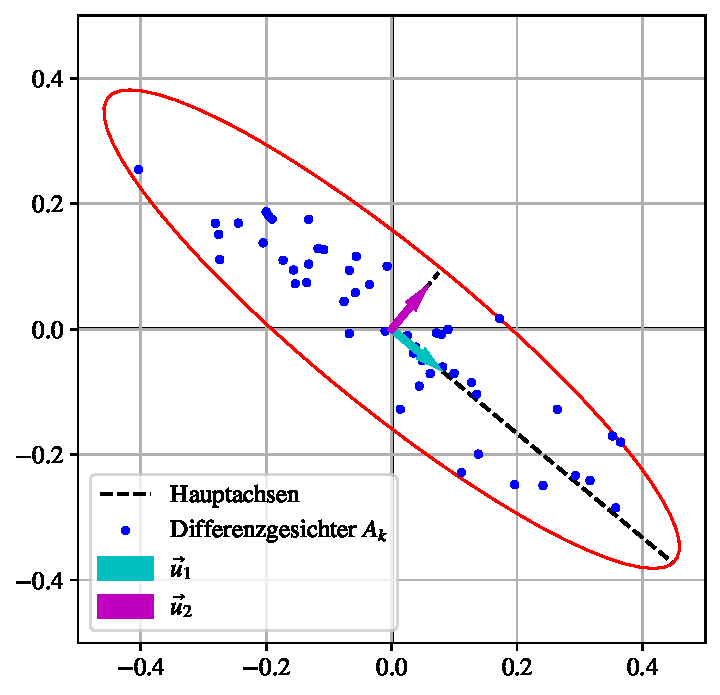
\includegraphics[width=0.45\textwidth]{images/facespace/principal_components} & 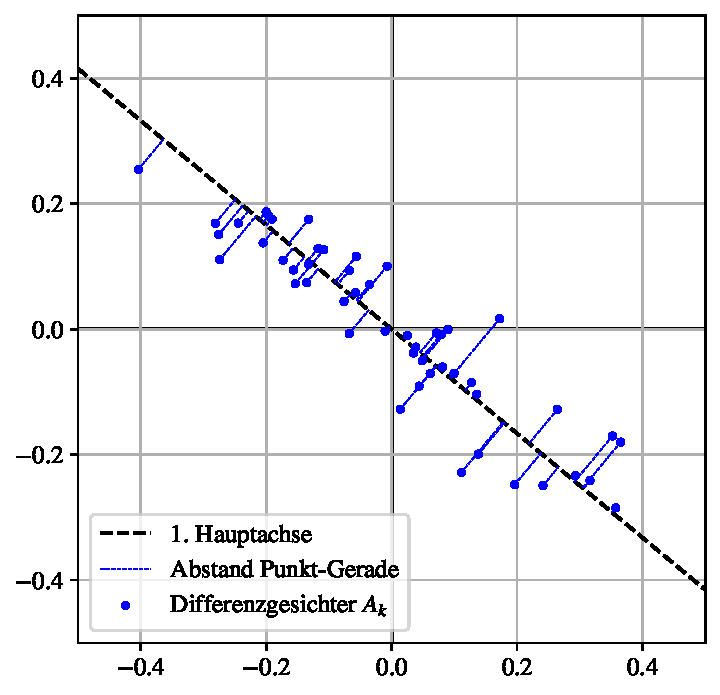
\includegraphics[width=0.45\textwidth]{images/facespace/distance_complicated} \\
	\end{tabular}
	\caption{Die Eigengesichter sind die orthonormalen Vektoren entlang den Hauptachsen.}
	\label{fig:construction}
\end{figure}

Wir werden nun das erste Eigengesicht $\vec{u}_1$ berechnen.
Dazu müssen wir zuerst verstehen was es bedeutet, einen Vektor \glqq{}entlang der grössten Streuung\grqq{} zu finden.
Die erste Hauptachse wird wie folgt bestimmt:
Sie ist diejenige Gerade, welche die Summe der Abstandsquadrate zu den Punkten $A_1,\ldots,A_K$ minimiert.
Dies ist rechts in Abbildung~\ref{fig:construction} gezeigt.
Um die Eigengesichter zu berechnen, müssen wir also den Abstand eines Punktes von einer Geraden berechnen können.
\begin{aufgabe} \label{aufg:distance_simple}
	\phantom{text}\\
	\begin{minipage}{0.55\textwidth}
		Berechnen Sie den Abstand des Punktes $A$ von der Geraden durch Null in Richtung $\vec{u}$, wobei $\vec{a}=\overrightarrow{OA}$ und
		\begin{align*}
			\vec{a}=
			\begin{pmatrix}
				1 \\
				-2
			\end{pmatrix},\quad
			\vec{u}=\frac{1}{5}
			\begin{pmatrix}
				4 \\
				-3
			\end{pmatrix}.
		\end{align*}
		\textit{Hinweis}: Der Vektor $\vec{u}$ hat Länge~1.
	\end{minipage}\hfill
	\begin{minipage}{0.4\textwidth}
		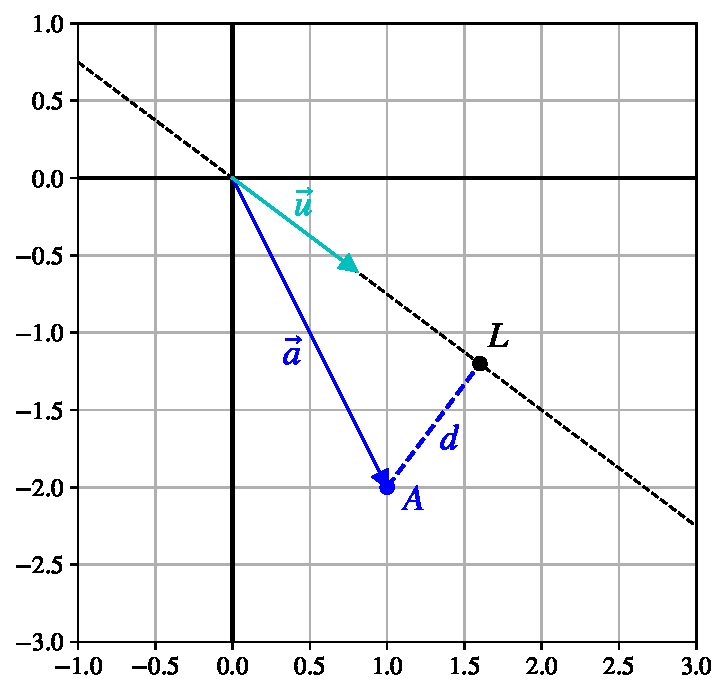
\includegraphics[width=\textwidth]{images/facespace/distance_simple}
	\end{minipage}
\end{aufgabe}
\begin{losung}
	Der Lotfusspunkt $L$ bezeichnet den Punkt auf der Geraden, welcher $A$ am nächsten liegt.
	Der Abstand von $L$ zum Ursprung ist $\vec{a}\cdot\vec{u}=2$.
	Dabei haben wir verwendet, dass $\vec{u}$ Länge 1 hat.
	Die gesuchte Distanz (blaue gestrichelte Linie im Bild) bezeichnen wir mit $d$.
	Nach dem Satz von Pythagoras gilt dann
	\begin{equation*}
		d^2+\left(\vec{a}\cdot\vec{u}\right)^2=\lVert\vec{a}\rVert^2.
	\end{equation*}
	Durch umformen erhalten wir
	\begin{equation*}
		d^2=\lVert\vec{a}\rVert^2-\left(\vec{a}\cdot\vec{u}\right)^2=5-4=1.
	\end{equation*}
	Der Abstand von $A$ zu Geraden ist also $d=1$.
\end{losung}
Was wir in Aufgabe~\ref{aufg:distance_simple} berechnet haben, funktioniert auch in höheren Dimensionen.
Seien $\vec v,\vec w\in\mathbb R^n$, wobei möglicherweise $n>3$.
Das Skalarprodukt dieser Vektoren ist dann definiert als
\begin{equation*}
	\vec v\cdot\vec w=v_1w_1+\ldots+v_nw_n.
\end{equation*}
Ganz analog ist auch das Quadrat Länge eines Vektors gegeben durch $\lVert\vec v\rVert^2=\vec v\cdot\vec v$.
Der Abstand eines Punktes zu einer Geraden berechnet sich dann nach der selben Formel wie in der Lösung von Aufgabe~\ref{aufg:distance_simple}.
\begin{aufgabe} \label{aufg:distance_complex}
	Sei $\vec{u}\in\mathbb R^{M\cdot N}$ ein Vektor der Länge~1.
	Dieser definiert die Gerade durch Null in Richtung $\vec{u}$.
	Finden Sie eine Formel für die Summe der Abstandsquadrate aller Differenzgesichter $A_1,\ldots,A_K$ zu dieser Geraden.
	Dies ist rechts in Abbildung~\ref{fig:construction} dargestellt.
\end{aufgabe}
\begin{losung}
	Wir konzentrieren uns zuerst auf ein beliebiges Differenzgesicht $\vec{a}_k=\overrightarrow{OA_k}$, wobei $1\leq k\leq K$.
	Dessen Abstand zur Geraden bezeichnen wir mit $d_k$.
	Analog zu Aufgabe~\ref{aufg:distance_simple} gilt
	\begin{equation*}
		d_k^2=\lVert\vec{a}_k\rVert^2-\left(\vec{a}_k\cdot\vec{u}\right)^2.
	\end{equation*}
	Die Summe dieser Abstandsquadrate $d_1^2+\ldots+d_K^2$ ist demnach gegeben durch
	\begin{equation*}
		\lVert\vec{a}_1\rVert^2-\left(\vec{a}_1\cdot\vec{u}\right)^2
		+\lVert\vec{a}_2\rVert^2-\left(\vec{a}_2\cdot\vec{u}\right)^2
		+\ldots+
		\lVert\vec{a}_{M\cdot N}\rVert^2-\left(\vec{a}_{M\cdot N}\cdot\vec{u}\right)^2.
	\end{equation*}
\end{losung}
Die Formel aus Aufgabe~\ref{aufg:distance_complex} liefert für jedes $\vec{u}$ einen positiven Wert.
Dasjenige $\vec{u}$, welches diesen Ausdruck minimiert, ist das erste Eigengesicht $\vec{u}_1$.
Die Eigengesichter zu berechnen, heisst also ein Minimierungsproblem zu lösen.
Dies ist nicht so einfach und ist daher bereits implementiert.

Die Eigengesichter wollen wir nun visualisieren, indem wir sie wieder als Bilder darstellen.
Doch da gibt es noch ein Problem.
Die Komponenten der Eigengesichter liegen nicht notwendigerweise in $\left[0,1\right]$ und können daher nicht als Graustufen interpretiert werden.
Damit man sie als Bilder darstellen kann, müssen wir deren Komponenten zuerst wie folgt nach $\left[0,1\right]$ abbilden.
Sei $\vec v\in\mathbb R^{M\cdot N}$ irgend ein Vektor, dessen Komponenten nicht notwendigerweise in $\left[0,1\right]$ liegen.
Sei $\min\left(\vec v\right)$ das Minimum und $\max\left(\vec v\right)$ das Maximum aller Komponenten von $\vec v$.
Wir betrachten nun den Vektor
\begin{equation*}
	\vec w=
	\begin{pmatrix}
		w_1 \\
		w_2 \\
		\vdots \\
		w_{M\cdot N}
	\end{pmatrix}
\end{equation*}
dessen Komponenten sich aus denen von $\vec v$ wie folgt zusammensetzen
\begin{equation*}
	w_i=\frac{v_i-\min\left(\vec v\right)}{\max\left(\vec v\right)-\min\left(\vec v\right)},
\end{equation*}
für alle $i\in\left\{1,\ldots,M\cdot N\right\}$.
Die Komponenten des Vektors $\vec w$ liegen dann alle in $\left[0,1\right]$.
Falls alle Komponenten von $\vec v$ gleich sind, ist $\min\left(\vec v\right)=\max\left(\vec v\right)$ und wir haben eine Division durch Null.
Wir ignorieren diesen Fall.
\begin{aufgabe} \label{aufg:scaling_theory}
	\phantom{text}
	\begin{enumerate}[label=(\alph*)]
		\item Betrachten Sie den Vektor
		\begin{equation*}
			\vec v=
			\begin{pmatrix}
				-2 \\
				4 \\
				1
			\end{pmatrix},
		\end{equation*}
		dessen Komponenten nicht alle in $\left[0,1\right]$ liegen.
		Berechnen Sie daraus den Vektor $\vec w$ gemäss obigem Verfahren.
		\item Begründen Sie, warum dieses Verfahren immer einen Vektor mit Komponenten in $\left[0,1\right]$ liefert, auch für einen allgemeinen Vektor $\vec v$.
	\end{enumerate}
\end{aufgabe}
\begin{losung}
	\phantom{text}
	\begin{enumerate}[label=(\alph*)]
		\item In obigem Beispiel ist $\min\left(\vec v\right)=-2$ und $\max\left(\vec v\right)=4$.
		Daraus ergibt sich für alle $i\in\left\{1,2,3\right\}$
		\begin{equation*}
			w_i=\frac{v_i-\left(-2\right)}{4-\left(-2\right)}=\frac{v_i+2}{6}.
		\end{equation*}
		Somit erhalten wir
		\begin{equation*}
			\vec w=
			\begin{pmatrix}
				0 \\
				1 \\
				\tfrac{1}{2}
			\end{pmatrix}.
		\end{equation*}
		\item Für alle Komponenten $v_i$ gilt stets
		\begin{equation*}
			\min\left(\vec v\right)\leq v_i\leq\max\left(\vec v\right).
		\end{equation*}
		Daraus folgt, dass im Bruch
		\begin{equation*}
			w_i=\frac{v_i-\min\left(\vec v\right)}{\max\left(\vec v\right)-\min\left(\vec v\right)},
		\end{equation*}
		der Nenner immer grösser oder Gleich dem Zähler ist, und dass beide nicht negativ werden können.
		Folglich muss $w_i\in\left[0,1\right]$ gelten.
	\end{enumerate}
\end{losung}
\begin{aufgabe} \label{aufg:scaling_code}
	Ergänzen Sie die Funktion \texttt{interpolate(v)}, welche den Vektor mit Komponenten in $\left[0,1\right]$ zurück gibt, der aus dem Vektor \texttt{v} durch obiges Verfahren entsteht.
	Testen Sie ihre Lösung mit dem Python Skript \texttt{plot\_eigenfaces.py}, welches ihre Funktion \texttt{interpolate(v)} auf die Eigengesichter $\vec u_1,\ldots,\vec u_K$ anwendet und diese als Bilder abspeichert.
	\textit{Hinweis:} Die Funktionen \texttt{np.min(v)} und \texttt{np.max(v)} liefern das Minimum und das Maximum eines Vektors \texttt{v}.
\end{aufgabe}
\begin{losung}
	Eine mögliche Lösung ist unten gezeigt.
	Die Eigengesichter sind in Abbildung~\ref{fig:eigenfaces} dargestellt.
\begin{lstlisting}[style=python]
import numpy as np

def interpolate(v):
	w = np.zeros_like(v)
	a = np.min(v)
	b = np.max(v)
	for vi, wi in zip(v, w):
		wi = (vi - a) / (b - a)
	return w
\end{lstlisting}
\end{losung}

\begin{figure}[ht]
	\centering
	\begin{tabular}{cccccccc}
		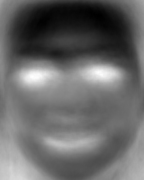
\includegraphics[width=0.1\textwidth]{images/eigenfaces/eigenface00} & 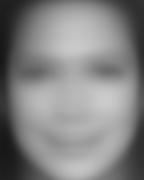
\includegraphics[width=0.1\textwidth]{images/eigenfaces/eigenface01} &
		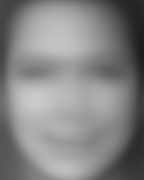
\includegraphics[width=0.1\textwidth]{images/eigenfaces/eigenface02} & 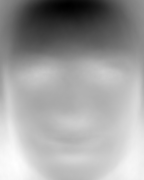
\includegraphics[width=0.1\textwidth]{images/eigenfaces/eigenface03} &
		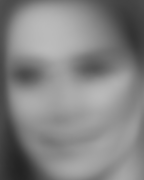
\includegraphics[width=0.1\textwidth]{images/eigenfaces/eigenface04} &
		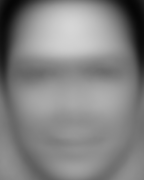
\includegraphics[width=0.1\textwidth]{images/eigenfaces/eigenface05} & 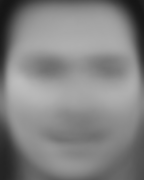
\includegraphics[width=0.1\textwidth]{images/eigenfaces/eigenface06} &
		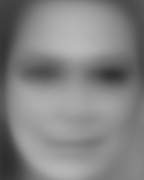
\includegraphics[width=0.1\textwidth]{images/eigenfaces/eigenface07} \\ \includegraphics[width=0.1\textwidth]{images/eigenfaces/eigenface08} &
		\includegraphics[width=0.1\textwidth]{images/eigenfaces/eigenface09} & \includegraphics[width=0.1\textwidth]{images/eigenfaces/eigenface10} &
		\includegraphics[width=0.1\textwidth]{images/eigenfaces/eigenface11} & \includegraphics[width=0.1\textwidth]{images/eigenfaces/eigenface12} &
		\includegraphics[width=0.1\textwidth]{images/eigenfaces/eigenface13} & \includegraphics[width=0.1\textwidth]{images/eigenfaces/eigenface14} &
		\includegraphics[width=0.1\textwidth]{images/eigenfaces/eigenface15} \\
	\end{tabular}
	\caption{Die ersten 16 Eigengesichter wurden wieder als Bild dargestellt.}
	\label{fig:eigenfaces}
\end{figure}

Im Grunde fangen die Eigengesichter charakteristische Gesichtszüge ein.
Mit charakteristisch ist hier gemeint, dass genau diese Gesichtszüge für die grösste Streuung unter allen Bildern der Datenbank verantwortlich sind.
Sie beschreiben die Merkmale, nach denen sich die Gesichter am meisten unterscheiden.
Besser gesagt: Das erste Eigengesicht fängt den Gesichtszug mit der grössten Streuung ein.
Die weiteren Eigengesichter fangen Gesichtszüge mit immer weniger Streuung ein.
Dies spiegelt sich auch in deren Konstruktion wieder, welche die Eigengesichter ja gerade als Vektoren entlang der grössten Streuung definiert.
\section{Projektion auf die Eigengesichter} \label{sec:eigenbasis}
\begin{tcolorbox}
	\centerline{\textbf{Lernziele Kapitel~\ref{sec:eigenbasis}}}
	\begin{enumerate}[leftmargin=*,label=\thesection.\arabic*]
		\item Die Eigenschaften \glqq{}orthogonal\grqq{} und \glqq{}orthonormal\grqq{} in $\mathbb R^n$ \textit{anwenden} können.
		\item Die Projektion eines Vektors auf einen Unterraum \textit{ausführen} können, wenn eine orthonormale Basis dieses Unterraumes gegeben ist.
	\end{enumerate}
\end{tcolorbox}
In diesem Unterkapitel wollen wir allgemeine Bilder als Linearkombination der Eigengesichter darstellen.
Man kann zeigen, dass alle Bilder der Datenbank exakt als Linearkombination der Eigengesichter geschrieben werden können.
Neue Bilder können im Allgemeinen mit so einer Linearkombination nur angenähert werden.
Die beste Näherung ist gerade die Projektion des neuen Bildes auf den Raum, der durch die Eigengesichter aufgespannt wird.
Was das genau bedeutet, wollen wir zuerst im $\mathbb R^3$ veranschaulichen.
\begin{figure}[ht]
	\centering
	\includegraphics[width=0.5\textwidth]{images/projection}
	\caption{Projektion $\vec a$ von $\vec p$ auf die Ebene durch Null, die von $\vec v_1$ und $\vec v_2$ aufgespannt wird. Der Vektor $\vec n$ steht normal auf die Ebene und es gilt $\vec p=\vec a+\vec n$.}
	\label{fig:projection}
\end{figure}
\begin{aufgabe} \label{aufg:projection_3d}
	Betrachten Sie die Vektoren
	\begin{equation*}
		\vec v_1=\frac{1}{\sqrt{3}}\begin{pmatrix}
			1 \\ 1 \\ 1
		\end{pmatrix},\quad
		\vec v_2=\frac{1}{\sqrt{2}}\begin{pmatrix}
			-1 \\ 1 \\  0
		\end{pmatrix},\quad
		\vec p=\begin{pmatrix}
			3 \\ 1 \\  2
		\end{pmatrix}.
	\end{equation*}
	\begin{enumerate}[label=(\alph*)]
		\item Sind die Vektoren $\vec v_1$ und $\vec v_2$ sind orthonormal? Begründen Sie.
		\item Die Vektoren $\vec v_1$ und $\vec v_2$ spannen eine Ebene durch den Nullpunkt auf.
		Berechnen Sie den Punkt $\vec a$, welcher der orthogonalen Projektion von $\vec p$ auf diese Ebene entspricht.
		Dazu können Sie zum Beispiel eine Zerlegung $\vec p=\vec a+\vec n$ wie in Abbildung~\ref{fig:projection} machen.
		\item Dann kann man $\vec a$ als Linearkombination vom $\vec v_1$ und $\vec v_2$ darstellen, also
		\begin{equation*}
			\vec a=c_1\vec v_1+c_2\vec v_2.
		\end{equation*}
		Berechnen Sie die Koeffizienten $c_1$ und $c_2$ in Termen von $\vec v_1,\vec v_2$ und $\vec p$.
	\end{enumerate}
\end{aufgabe}
\begin{losung*}
	\phantom{text}
	\begin{enumerate}[label=(\alph*)]
		\item Die Vektoren sind orthonormal. Wir berechnen das Skalarprodukt
		\begin{equation*}
			\vec v_1\cdot\vec v_2= \frac{1}{\sqrt{3}}\cdot\frac{1}{\sqrt{2}}\cdot\left(1\cdot\left(-1\right)+1\cdot 1+1\cdot 0\right)=0.
		\end{equation*}
		Die beiden Vektoren sind also orthogonal.
		Es bleibt zu zeigen, dass sie beide Länge 1 haben. In der Tat gilt
		\begin{equation*}
			\vec v_1\cdot\vec v_1=\frac{1}{3}\left(1^2+1^2+1^2\right)=1
		\end{equation*}
		und
		\begin{equation*}
			\vec v_2\cdot\vec v_2=\frac{1}{2}\left(\left(-1\right)^2+1^2+0^2\right)=1.
		\end{equation*}
		\item Wir zerlegen $\vec p=\vec a+\vec n$ wie in Abbildung~\ref{fig:projection} in einen Vektor $\vec a$ der in der Ebene liegt und einen Vektor $\vec n$ der orthogonal zur Ebene steht.
		Gesucht ist der Vektor $\vec a$.
		Da er in der Ebene liegt, gibt es eindeutige Koeffizienten $c_1$ und $c_2$, so dass
		\begin{equation*}
			\vec a=c_1\vec v_1+c_2\vec v_2.
		\end{equation*}
		Wir addieren $\vec n$ auf beiden Seiten und erhalten
		\begin{equation*}
			\vec p=c_1\vec v_1+c_2\vec v_2+\vec n.
		\end{equation*}
		Nun bilden wir auf beiden Seiten das Skalarprodukt mit $\vec v_1$, also
		\begin{equation*}
			\vec v_1\cdot\vec p=c_1\underbrace{\vec v_1\cdot\vec v_1}_{=1}+c_2\underbrace{\vec v_1\cdot\vec v_2}_{=0}+\underbrace{\vec v_1\cdot\vec n}_{=0}.
		\end{equation*}
		Hier haben wir verwendet, dass $\vec v_1$ orthogonal ist zu $\vec v_2$ und $\vec n$.
		Wir erhalten
		\begin{equation*}
			c_1=\vec v_1\cdot\vec p=\frac{6}{\sqrt{3}}.
		\end{equation*}
		In dem man stattdessen auf beiden Seiten das Skalarprodukt mit $\vec v_2$ bildet, erhält man analog
		\begin{equation*}
			c_2=\vec v_2\cdot\vec p=-\frac{2}{\sqrt{2}}.
		\end{equation*}
		Damit berechnen wir die Projektion
		\begin{equation*}
			\vec a
			=c_1\vec v_1+c_2\vec v_2
			=2\begin{pmatrix}
				1 \\ 1 \\ 1
			\end{pmatrix}
			-2\begin{pmatrix}
				-1 \\ 1 \\ 0
			\end{pmatrix}
			=\begin{pmatrix}
				4 \\ 0 \\ 2
			\end{pmatrix}.
		\end{equation*}
		\item In der Lösung der vorherigen Teilaufgabe haben wir die Koeffizienten schon berechnet zu
		\begin{equation*}
			c_1=\frac{6}{\sqrt{3}}
			\quad\quad\text{und}\quad\quad
			c_2=-\frac{2}{\sqrt{2}}.
		\end{equation*}
	\end{enumerate}
\end{losung*}

Was wir in der vorherigen Teilaufgabe berechnet haben, funktioniert auch in höheren Dimensionen.
Seien $\vec u,\vec v\in\mathbb R^n$, wobei möglicherweise $n>3$.
Das Skalarprodukt dieser Vektoren ist dann definiert als
\begin{equation*}
	\vec u\cdot\vec v=u_1v_1+\ldots+u_nv_n,
\end{equation*}
wobei $u_1,\ldots,u_n$ die Komponenten von $\vec u$ und $v_1,\ldots,v_n$ die Komponenten von $\vec v$ sind.
Wir sagen, die beiden Vektoren sind orthogonal, wenn $\vec u\cdot\vec v=0$.
Falls sie zusätzlich Länge 1 haben, also $\vec u\cdot\vec u=1$ und $\vec v\cdot\vec v=1$, dann heissen sie orthonormal.
Eine Familie $\vec v_1,\ldots,\vec v_K\in\mathbb R^n$ heisst orthonormal, wenn die Vektoren alle paarweise orthonormal sind.
Sie spannen dann einen $K$-dimensionalen Raum auf.
Wir können wie in der Aufgabe die Projektion eines Vektors $\vec p\in\mathbb R^n$ auf diesen Raum berechnen, nämlich
\begin{equation*}
	c_1\vec v_1+\ldots+c_n\vec v_n,
\end{equation*}
wobei die Koeffizienten gegeben sind durch
\begin{equation*}
	c_i=\vec v_i\cdot p
\end{equation*}
für alle $i\in\left\{1,\ldots,n\right\}$.

Nun betrachten wir wieder die Eigengesichter $\vec u_1,\ldots,\vec u_K$.
Gemäss der Konstruktion aus dem letzten Kapitel sind diese orthonormal.
Wir betrachten zudem die Mona Lisa von Leonardo da Vinci, ein Bild das nicht in unserer Datenbank ist.
Den entsprechenden Vektor nennen wir $\vec p\in\mathbb R^{M\cdot N}$.
Um dieses Bild in den Raum der Differenzgesichter zu verschieben, müssen wir noch das Durchschnittsgesicht $\vec m$ subtrahieren.
Das entstehende Differenzgesicht kann dann näherungsweise als Linearkombination der Basis $\vec a_1,\ldots,\vec a_K$ oder auch der Basis der Eigengesichter $\vec u_1,\ldots,\vec u_K$ dargestellt werden.
Letzteres geht mit einer Projektion wie oben beschrieben.
\begin{aufgabe} \label{aufg:projection}
	Sei $\vec p\in\mathbb R^{M\cdot N}$ das Bild der Mona Lisa und $\vec u_1,\ldots,\vec u_K\in\mathbb R^{M\cdot N}$ die Eigengesichter.
	Berechnen Sie die Koeffizienten $c_1,\ldots,c_K$ der Projektion von $\vec p-\vec m$ auf die Eigengesichter.
	Geben Sie die Koeffizienten in Termen von $\vec p, \vec m$ und den Eigengesichtern an.
\end{aufgabe}
\begin{losung*}
	Wie in der letzten Aufgabe verwenden wir, das die Eigengesichter orthonormal sind.
	Wir bilden das Skalarprodukt beider Seiten der obigen Gleichung mit $u_1$, also
	\begin{equation*}
		\vec u_1\cdot\left(\vec p-\vec m\right)=c_1\underbrace{\vec u_1\cdot\vec u_1}_{=1}+c_2\underbrace{\vec u_1\cdot\vec u_2}_{=0}+\ldots+c_K\underbrace{\vec u_1\cdot\vec u_K}_{=0}.
	\end{equation*}
	Wenn wir das auch noch mit $\vec u_2,\ldots,\vec u_K$ machen erhalten wir
	\begin{equation*}
		\vec u_k\cdot\left(\vec p-\vec m\right)=c_k,
	\end{equation*}
	für alle $k\in\{1,\ldots,K\}$.
\end{losung*}

Hat man die Koeffizienten der Linearkombination berechnet, so kann die Projektion der Mona Lisa wieder als Linearkombination der Eigengesichter und des Durchschnittsgesichtes darstellen
\begin{equation*}
	\vec m+c_1\vec u_1+c_2\vec u_2+\ldots+c_Ku_K.
\end{equation*}
\begin{aufgabe} \label{aufg:compute_coefficients}
	Seien \texttt{p} und \texttt{m} Vektoren der Länge $M\cdot N$, wobei \texttt{p} ein Gesicht zeigt (z.B. das der Mona Lisa) und \texttt{m} das Durchschnittsgesicht ist.
	Sei zudem \texttt{u\_list} die Liste der Eigengesichter.
	Ergänzen Sie die Funktion \texttt{compute\_coefficients(p, m, u\_list)}, welche die Liste der Koeffizienten der Linearkombination aus Abbildung~\ref{fig:eigen_basis} zurück gibt.
	Um Ihre Lösung zu testen können Sie das Python Skript \texttt{basis\_expansion.py} laufen lassen, welches die Projektion der Mona Lisa mit den von Ihnen berechneten Koeffizienten darstellt.
	\textit{Hinweis:} Mit \texttt{np.dot(v,w)} lässt sich das Skalarprodukt zweier Vektoren \texttt{v} und \texttt{w} berechnen.
\end{aufgabe}
\begin{losung*}
	Die Lösung könnte zum Beispiel so aussehen.\\[0.5cm]
	\begin{minipage}{0.65\textwidth}
\begin{lstlisting}[style=python]
import numpy as np

def compute_coefficients(p, m, u_list):
	K = len(u_list)
	c_list = np.empty((K,))
	for c, u in zip(c_list, u_list):
		c = np.dot(u, p - m)
	return c_list
\end{lstlisting}
	\end{minipage}\hfill
	\begin{minipage}{0.35\textwidth}\vspace{-1cm}
		\centering Rekonstruktion:\\[0.5cm]
		\includegraphics[width=0.4\textwidth]{images/eigenfaces/mona_lisa_eigen_approx}
	\end{minipage}
\end{losung*}

Anscheinend sieht die Projektion fast gleich aus wie das Bild selber.
Etwas informell ist das in in Abbildung~\ref{fig:eigen_basis} dargestellt.
\begin{figure}[ht]
	\centering
	\begin{tabular}{m{1.8cm} c c c c c m{2cm} c c c m{2cm} c c}
		\includegraphics[width=0.1\textwidth]{images/eigenfaces/mona_lisa_eigen_approx} &
		$=$ & $\vec m$ & $+$ & $c_1$ & $\cdot$ & \includegraphics[width=0.1\textwidth]{images/eigenfaces/eigenface00}
		& $+$ & $c_2$ & $\cdot$ & \includegraphics[width=0.1\textwidth]{images/eigenfaces/eigenface01} & $+$ & $\cdots$
	\end{tabular}
	\caption{Projektion der Mona Lisa auf die Eigengesichter.}
	\label{fig:eigen_basis}
\end{figure}
Dieses Phänomen bedeutet, dass die Mona Lisa ganz oder in sehr guter Näherung im Raum liegt, er durch die Eigengesichter aufgespannt wird.
In Abbildung~\ref{fig:projection} würde das einem $\vec p$ entsprechen, dass mit der Ebene einen verschwindend kleinen Winkel einschliesst, also fast in der Ebene liegt.
Mit dieser Beobachtung wollen wir und im nächsten Kapitel genauer auseinandersetzen.
\section{Bildkompression} \label{sec:compression}
\begin{tcolorbox}
	\centerline{\textbf{Lernziele Kapitel~\ref{sec:compression}}}
	\begin{enumerate}[leftmargin=*,label=\thesection.\arabic*]
		\item \label{item:compression_theory} Die Lernenden können erklären, was die Eigengesichter im Vergleich zu anderen Basen auszeichnet und warum sie sich zur Bildkompression eignen.\\
		(Aufgaben~\ref{aufg:coef} und~\ref{aufg:compression_theory})
		\item \label{item:compression_code} Die Lernenden können mit gegebenen Eigengesichtern eine Bildkompression in Python durchführen, falls alle Bilder als Vektoren gegeben sind.\\
		(Aufgabe~\ref{aufg:compression})
	\end{enumerate}
\end{tcolorbox}
Wenn wir ein schwarz-weiss Bild mit der Auflösung $M=144$ mal $N=180$ Pixel für Pixel abspeichern, so müssen wir $M\cdot N=25920$ Zahlen abspeichern.
Unter Bildkompression versteht man Verfahren, die Bilder mit weniger Zahlen darstellen können.
Das ist zum Beispiel nützlich wenn man Bilder über das Internet verschicken möchte (oder gleich ganze Filme).
Die Datenmenge kann durch Kompression stark verringert werden, was zu viel kürzeren Download-Zeiten führt.
Mit den Eigengesichtern lassen sich Bilder von Gesichtern komprimieren.
Grund dafür ist eine spezielle Eigenschaft, welche die Eigengesichter auszeichnet, und dir wir nun untersuchen werden.

Im letzten Kapitel haben wir das Gemälde der Mona Lisa durch eine Projektion als Linearkombination der Eigengesichter und es Durchschnittsgesichtes angenähert.
Dazu mussten wir mit geeigneten Skalarprodukten die Koeffizienten $c_1,\ldots,c_K$ dieser Linearkombination berechnen.
Allerdings hätte man anstatt der Eigengesichter auch direkt die Differenzgesichter $\vec a_1,\ldots,\vec a_K$ der Bilder aus der Datenbank nehmen können.
In diesem Fall würde man einfach andere Koeffizienten erhalten.
Allerdings lassen sich diese nicht so einfach berechnen, da diese Differenzgesichter nicht orthonormal sind.
Man betrachte Abbildung~\ref{fig:mona_lisa_reconstruction} für einen Vergleich der beiden Varianten.
\begin{figure}[ht]
	\centering
	\begin{tabular}{lcr}
		\includegraphics[width=0.2\textwidth]{images/eigenfaces/mona_lisa_naive_approx} &
		\includegraphics[width=0.2\textwidth]{images/eigenfaces/mona_lisa_original} & \includegraphics[width=0.2\textwidth]{images/eigenfaces/mona_lisa_eigen_approx}
	\end{tabular}
	\caption{Rekonstruktion der Mona Lisa. Links wurden die Differenzbilder der Testgesichter $\vec a_1,\ldots,\vec a_K$ verwendet. Rechts wurden die Eigengesichter $\vec u_1,\ldots,\vec u_K$ verwendet. In der Mitte ist das Original.}
	\label{fig:mona_lisa_reconstruction}
\end{figure}
Ein weiterer Unterschied zwischen diesen beiden Ansätzen ist die Verteilung der Beträge der Koeffizienten, also $\lvert c_1\rvert,\ldots,\lvert c_K\rvert$.
Diese sind in Abbildung~\ref{fig:coef} gezeigt.
\begin{figure}[ht]
	\centering
	\begin{tabular}{lr}
		\includegraphics[width=0.45\textwidth]{images/eigenfaces/naive_coef} & \includegraphics[width=0.45\textwidth]{images/eigenfaces/eigen_coef} \\
	\end{tabular}
	\caption{Der Absolutbetrag der Koeffizienten der Linearkombination des Differenzgesichtes der Mona Lisa, die in Abbildung~\ref{fig:mona_lisa_reconstruction} verwendet wurden. Links die Differenzgesichter der Datenbank und rechts die Eigengesichter verwendet.}
	\label{fig:coef}
\end{figure}
\begin{aufgabe} \label{aufg:coef}
	Betrachten Sie die Abbildung~\ref{fig:coef}, welche die Koeffizienten der Linearkombinationen zeigt, die für die Bilder links bzw. rechts in Abbildung~\ref{fig:mona_lisa_reconstruction} verwendet wurden.
	Beschreiben Sie die Unterschiede in der Verteilung der Koeffizienten.
	Welche Rückschlüsse kann man dadurch ziehen?
\end{aufgabe}
\begin{losung}
	Die Koeffizienten der Eigengesichter fallen schnell ab.
	Dem rechten Bild kann man entnehmen, dass ungefähr die ersten 2000 Eigengesichter fast den ganzen Beitrag zur Linearkombination leisten.
	Die Koeffizienten der restlichen Eigengesichter ist fast Null.
	Bei der Basis der Differenzgesichter ist keine solche Struktur zu erkennen.
	Es ist nicht auszumachen, ob und welche Differenzgesichter besonders stark vertreten sind.
\end{losung}
Was wir hier in Abbildung~\ref{fig:coef} beobachtet haben ist kein Einzelfall.
Obwohl wir nur das Beispiel der Mona Lisa betrachtet haben, würden andere Gesichter ähnlich verteilte Koeffizienten liefern.
Die Lösung der vorherigen Aufgabe ist zugleich die Grundidee der Bildkompression mittels Eigengesichter.
Anstatt alle der $K$ Eigengesichter, verwendet man nur die ersten $\tilde K$ Eigengesichter um ein Bild darzustellen.
Die Abbildung~\ref{fig:coef} lässt vermuten, dass wenn $\tilde K$ gross genug gewählt ist, aber immer noch viel kleiner als $K$, sich die Bildqualität nicht wesentlich verschlechtert.
Genauer gesagt, können wir ablesen, dass wohl die ersten $\tilde K=2000$ Eigengesichter ausreichend sein sollten.
Nun wollen ein Bild $\vec p$ rekonstruieren, indem wir nur die ersten $\tilde K$ Eigengesichter verwenden.
Das rekonstruierte Gesicht bezeichnen wir mit $\vec a$, also
\begin{equation*}
	\vec a=\vec m+c_1\vec u_1+c_2\vec u_2+\ldots+c_{\tilde K}\vec u_{\tilde K},
\end{equation*}
wobei $\tilde K\leq K$ und $\vec u_1,\ldots,\vec u_{\tilde K}$ sind die ersten $\tilde K$ Eigengesichter.
Wie man die Koeffizienten $c_1,\ldots,c_{\tilde K}$ berechnet, haben wir im letzten Kapitel gesehen.
\begin{aufgabe} \label{aufg:compression}
	Ergänzen Sie im Skript \texttt{chapter6.py} die Funktion \texttt{compress(p, m, u\_list, K\_tilde)}, welche einen Vektor der Länge $M\cdot N$ zurück gibt, der dem Bild $\vec a$ entspricht.
	Hier bezeichnen \texttt{p} das ursprüngliche Bild $\vec p$ und \texttt{m} das Durchschnittsgesicht $\vec m$.
	Die Liste \texttt{u\_list} enthält die Eigengesichter und \texttt{K\_tilde} entspricht der Anzahl $\tilde K$ der Eigengesichter, die verwendet werden sollen.
	Testen Sie ihre Lösung indem Sie das Skript \texttt{chapter6.py} laufen lassen, welches die rekonstruierten Bilder ausgibt.
	Dazu müssen Sie in der Kommandozeile den Pfad zum File \texttt{eigenfaces.dat} übergeben.
	\textit{Hinweis:} Verwenden Sie in ihrem Code die Funktion \texttt{compute\_coefficients(p, m, u\_list)} aus Aufgabe~\ref{aufg:compute_coefficients}.
\end{aufgabe}
\begin{losung}
	Die Lösung könnte zum Beispiel so aussehen.
\inputminted[frame=single,framesep=5pt,firstline=5,lastline=12]{python}{codes/solution/chapter6.py}
Die durch \texttt{chapter6.py} generierten Bilder sind in Abbildung~\ref{fig:compression} gezeigt.
\end{losung}
\begin{figure}[ht]
	\centering
	\begin{tabular}{cccc}
		$\tilde K=20$ & $\tilde K=200$ & $\tilde K=2000$ & Original \\
		\includegraphics[width=0.1\textwidth]{images/compression/mona_lisa_20} &
		\includegraphics[width=0.1\textwidth]{images/compression/mona_lisa_200} &
		\includegraphics[width=0.1\textwidth]{images/compression/mona_lisa_2000} & \includegraphics[width=0.1\textwidth]{images/compression/mona_lisa} \\
		\includegraphics[width=0.1\textwidth]{images/compression/queen_elizabeth_20} &
		\includegraphics[width=0.1\textwidth]{images/compression/queen_elizabeth_200} &
		\includegraphics[width=0.1\textwidth]{images/compression/queen_elizabeth_2000} & \includegraphics[width=0.1\textwidth]{images/compression/queen_elizabeth} \\
		\includegraphics[width=0.1\textwidth]{images/compression/chair_20} &
		\includegraphics[width=0.1\textwidth]{images/compression/chair_200} &
		\includegraphics[width=0.1\textwidth]{images/compression/chair_2000} & \includegraphics[width=0.1\textwidth]{images/compression/chair} \\
		\includegraphics[width=0.1\textwidth]{images/compression/columbia_20} &
		\includegraphics[width=0.1\textwidth]{images/compression/columbia_200} &
		\includegraphics[width=0.1\textwidth]{images/compression/columbia_2000} & \includegraphics[width=0.1\textwidth]{images/compression/columbia}
	\end{tabular}
	\caption{Rekonstruktion mit verschiedenen $\tilde K$. Gezeigt sind die Mona Lisa, Queen Elizabeth, ein Stuhl und das erste Space Shuttle \glqq{}Columbia\grqq{}. Gesichter werden generell besser rekonstruiert als andere Bilder.}
	\label{fig:compression}
\end{figure}
Was wir in Abbildung~\ref{fig:compression} beobachten ist eine Bildkompression.
Sind die Eigengesichter bekannt, so lässt sich ein Bild rekonstruieren aus den Koeffizienten $c_1,\ldots,c_{\tilde K}$ der ersten $\tilde K$ Eigengesichter.
Um ein Bild eines Gesichtes in leicht verminderter Qualität über das Internet zu versenden, wäre es ausreichend, nur $\tilde K=2000$ Zahlen zu versenden, sofern der Empfänger über die Eigengesichter verfügt.
Wir erinnern uns, dass ein Bild welches Pixelweise versendet wird, $M\cdot N=25920$ Zahlen benötigt.
Das ist etwa ein Faktor 13 mehr als die komprimierte Variante.
Trotzdem sieht man für $\tilde K=2000$ kaum einen Unterschied zum Original in Abbildung~\ref{fig:compression}.
Gleichzeitig sehen wir, dass die aggressivere Komprimierung mit $\tilde K=200$ die Bildqualität doch sehr vermindert.
Aber das konnte man aufgrund des rechten Verteilung in Abbildung~\ref{fig:coef} schon vermuten.
Weiter beobachten wir, dass die Komprimierung für Bilder, welche kein Gesicht zeigen, weniger gut funktioniert.
Der Grund dafür ist, das diese Differenzbilder nicht notwendigerweise nahe am Raum liegen, der durch die Differenz\textbf{gesichter} der Datenbank aufgespannt wird.
Doch die Eigengesichter sind eine Basis eben dieses Unterraumes.
\begin{aufgabe} \label{aufg:compression_theory}
	Könnte man für die Bildkompression anstelle der Eigengesichter auch die Differenzgesichter $\vec{a}_1,\ldots,\vec{a}_K$ nehmen?
	\textit{Hinweis}: Betrachten Sie Abbildung~\ref{fig:coef}.
\end{aufgabe}
\begin{losung}
	Nein, bei den Differenzgesichter ist nicht klar, welche Vektoren weggelassen werden können.
	Selbst wenn für ein konkretes Bild einige wenige ausreichen würden, so gibt es keine Möglichkeit zu bestimmen, welche das sind.
	Zudem sind diese Vektoren nicht orthonormal.
	Daher ist die Berechnung der Koeffizienten nur mittels Skalarprodukt nicht möglich.
\end{losung}

%\section{Geschlechtserkennung} \label{sec:binary}
Im letzten Kapitel haben wir die Bildkompression mittels Eigengesichter kennengelernt.
Diese eröffnet viele neue Möglichkeiten.
Eine davon ist die \textit{Geschlechtserkennung}.
Damit ist gemeint, dass man zu einem gegebenen Gesicht $\vec p\in\mathbb R^{M\times N}$ entscheidet, ob es einen Mann oder eine Frau zeigt.
Dazu verwenden wir ein bekanntes Konzept aus der Vektorgeometrie, die Ebene, oder genauer gesagt, die Hyperebene.
\section{Gesichtserkennung} \label{sec:recognition}
\begin{tcolorbox}
	\centerline{\textbf{Lernziele Kapitel~\ref{sec:recognition}}}
	\begin{enumerate}[leftmargin=*,label=\thesection.\arabic*]
		\item \label{item:recognition} Die Lernenden können erklären, wie die Eigengesichter das \glqq{}ähnlich aussehen\grqq{} von Gesichtern quantifizieren können.\\
		(Aufgaben~\ref{aufg:quantification} und~\ref{aufg:quantification_code})
	\end{enumerate}
\end{tcolorbox}
Nun wollen wir die Eigengesichter nutzen für eine Gesichtserkennung nutzen.
Wie bereits in der Einleitung erklärt, ist Gesichtserkennung im Grunde eine Klassifizierung.
Hier als Beispiel betrachten wir 8 verschiedene Klassen.
\begin{table}[ht]
	\centering
	\begin{tabular}{|c|c|c|c|}
		\hline
		Daniel Radcliffe & Emma Stone & Emma Watson & Eva Green \\
		\includegraphics[width=0.2\textwidth]{images/recognition/Daniel_Radcliffe} & \includegraphics[width=0.2\textwidth]{images/recognition/Emma_Stone} & \includegraphics[width=0.2\textwidth]{images/recognition/Emma_Watson} & \includegraphics[width=0.2\textwidth]{images/recognition/Eva_Green} \\ \hline
		Jennifer Lawrence & Orlando Bloom & Pierce Brosnan & Tom Cruise \\
		\includegraphics[width=0.2\textwidth]{images/recognition/Jennifer_Lawrence} & \includegraphics[width=0.2\textwidth]{images/recognition/Orlando_Bloom} & \includegraphics[width=0.2\textwidth]{images/recognition/Pierce_Brosnan} & \includegraphics[width=0.2\textwidth]{images/recognition/Tom_Cruise} \\ \hline
	\end{tabular}
	\caption{Die acht verschiedenen Klassen. }
	\label{tab:classes}
\end{table}
Wir verwenden in diesem Kapitel eine Datenbank die nur aus Bilder dieser 8 Personen besteht.
Diese kann hier heruntergeladen werden
\begin{center}
	\url{https://people.math.ethz.ch/~rioliver/eigenfaces/datenbank_small.zip}
\end{center}
Sie enthält von jeder Person genau 10 Bilder.
Das heisst, sie besteht aus $K=8\cdot 10=80$ Bildern.
Pro Klasse haben wir zusätzlich 3 Testbilder.
Das sind Bilder die zwar jeweils eine dieser 8 Personen zeigen, aber nicht in der Datenbank enthalten sind.
Das Ziel ist nun die Testbilder möglichst der richtigen Klasse zuzuordnen.
So können wir unsere Gesichtserkennung testen, daher der Name \glqq{}Testbilder\grqq{}.
\begin{figure}[ht]
	\centering
	\begin{tabular}{|c m{2cm} m{2cm} m{2cm} m{2cm} m{2cm}|}
		\hline
		Datanbank &
		\includegraphics[width=0.1\textwidth]{images/recognition/training_faces/training_0} &
		\includegraphics[width=0.1\textwidth]{images/recognition/training_faces/training_1} &
		\includegraphics[width=0.1\textwidth]{images/recognition/training_faces/training_2} &
		\includegraphics[width=0.1\textwidth]{images/recognition/training_faces/training_3} &
		\includegraphics[width=0.1\textwidth]{images/recognition/training_faces/training_4} \\
		&
		\includegraphics[width=0.1\textwidth]{images/recognition/training_faces/training_5} &
		\includegraphics[width=0.1\textwidth]{images/recognition/training_faces/training_6} &
		\includegraphics[width=0.1\textwidth]{images/recognition/training_faces/training_7} &
		\includegraphics[width=0.1\textwidth]{images/recognition/training_faces/training_8} &
		\includegraphics[width=0.1\textwidth]{images/recognition/training_faces/training_9} \\ \hline
		Testbilder &
		\includegraphics[width=0.1\textwidth]{images/recognition/test_faces/test_0} &
		\includegraphics[width=0.1\textwidth]{images/recognition/test_faces/test_1} &
		\includegraphics[width=0.1\textwidth]{images/recognition/test_faces/test_2} &
		& \\ \hline
	\end{tabular}
	\caption{Datenbank- und Testbilder am Beispiel der Klasse \glqq{}Daniel Radcliffe\grqq{}}
	\label{fig:testfaces}
\end{figure}
Zwar ist das für einen Menschen ganz leicht, aber für einen Computer ist das überhaupt nicht einfach.
Im Grunde müssen wir den Computer lehren, wann zwei Bilder ähnlich aussehen.
Dazu brauchen wir ein Mass für die Distanz zweier Bilder.
Es stellt sich heraus, dass die Eigengesichter ein Solches liefern.
Seien nun $\vec p$ und $\vec q$ zwei Bilder von Gesichtern.
Wir schreiben die entsprechenden Differenzgesichter als Linearkombination der Eigengesichter
\begin{equation*}
	\vec p-\vec m=c_1\vec u_1+c_2\vec u_2+\ldots+c_K\vec u_K
\end{equation*}
und
\begin{equation*}
	\vec q-\vec m=\tilde c_1\vec u_1+\tilde c_2\vec u_2+\ldots+\tilde c_K\vec u_K,
\end{equation*}
wobei nun $K=80$ und $\vec m$ das Durchschnittsgesicht der Bilder der neuen Datenbank ist.
Entsprechend sehen die Eigengesichter auch etwas anders aus, aber deren Eigenschaften sind die selben.
Das besagte Mass der Distanz zwischen den Gesichtern $\vec p$ und $\vec q$ definieren wir als
\begin{equation*}
	D\left(\vec p,\vec q\right)=\left(c_1-\tilde c_1\right)^2+\left(c_2-\tilde c_2\right)^2+\ldots+\left(c_K-\tilde c_K\right)^2.
\end{equation*}
\begin{aufgabe} \label{aufg:quantification}
	Warum entspricht dieser Begriff von Distanz dem \glqq{}Ähnlich aussehen\grqq{} von Gesichtern?
	Erklären Sie in Worten.
	\textit{Hinweis:} Rufen Sie sich die Konstruktion der Eigengesichter und die Diskussion am Ende von Kapitel~\ref{sec:facespace} in Erinnerung.
\end{aufgabe}
\begin{losung}
	Die Eigengesichter fangen gewisse Gesichtszüge ein.
	Die Funktion $D\left(\vec p,\vec q\right)$ vergleicht, wie fest sich $\vec p$ und $\vec q$ in eben diesen Gesichtszügen unterscheiden.
	Dabei werden die ersten Eigengesichter am stärksten gewichtet, da ihre Koeffizienten typischerweise am grössten sind (Abbildung~\ref{fig:coef}).
	Das macht auch Sinn, denn es sind genau die ersten Eigengesichter (Gesichtszüge), in denen sich die Gesichter der Datenbank am meisten unterscheiden.
	Die Bilder nur Pixel für Pixel zu vergleichen macht keinen Sinn, denn kein Pixel kann alleine eine Information über ein Gesicht tragen.
	Anders gesagt können sich zwei Bilder in jedem Pixel stark unterscheiden und dennoch die selbe Person zeigen.
	Mit Gesichtszügen ist dies kaum möglich.
\end{losung}
Sei nun ein Bild $\vec p$ gegeben, das nicht notwendigerweise in der Datenbank enthalten ist.
Das Bild soll zudem eine der 8 Personen aus Tabelle~\ref{tab:classes} zeigen.
Jedoch wissen wir nicht welche.
Wir werden versuchen das mit folgendem Verfahren zu erraten.
\begin{enumerate}[leftmargin=3cm, label=Schritt \arabic*:]
	\item Seien $\vec q_1,\ldots,\vec q_{80}$ die Bilder der Datenbank.
	Wir berechnen die Distanz $D\left(\vec p,\vec q_i\right)$ für $i=1,\ldots,80$.
	\item Eines dieser Bilder wird die kleinste Distanz zu $\vec p$ haben, sagen wir das ist $\vec q_j$ für ein bestimmtes $1\leq j\leq 80$.
	\item Wir schauen in der Datenbank nach, welche Person auf dem Bild $\vec q_j$ gezeigt ist. Da $\vec p$ ähnlich aussieht, zeigt es wohl die selbe Person und wir klassifizieren $\vec p$ entsprechend.
\end{enumerate}
\begin{aufgabe} \label{aufg:quantification_code}
	Ergänzen Sie im Skript \texttt{chapter7.py} die Funktion \texttt{distance(p, q, m, u\_list)} welche die Distanz $D\left(\vec p,\vec q\right)$ zweier Bilder zurück gibt.
	Dabei ist \texttt{m} das Durchschnittsgesicht und \texttt{u\_list} enthält die Liste der Eigengesichter.
	Die Variablen \texttt{p} und \texttt{q} enthalten die Vektoren $\vec p$ und $\vec q$.
	Testen Sie ihre Implementation indem Sie das Skript \texttt{chapter7.py} ausführen.
	Dazu müssen Sie in der Kommandozeile den Pfad zur reduzierten Datenbank angeben.
	\textit{Hinweis:} Verwenden sie die Funktion \texttt{compute\_coefficients(...)} aus Aufgabe~\ref{aufg:compute_coefficients}.
\end{aufgabe}
\begin{losung}
	Die Lösung könnte zum Beispiel so aussehen.
\inputminted[frame=single,framesep=5pt,firstline=5,lastline=9]{python}{codes/solution/chapter7.py}
	Der Output von \texttt{recognition.py} ist in Tabelle~\ref{tab:recognition} gelistet.
\end{losung}
\begin{table}[ht]
	\centering
	\begin{tabular}{|l|c|c|}
		\hline
		\textbf{Klasse} & \textbf{Anzahl Testbilder} & \textbf{davon richtig klassifiziert} \\ \hline
		Daniel Radcliffe & 3 & 2 \\ \hline
		Emma Stone & 3 & 2 \\ \hline
		Emma Watson & 3 & 2 \\ \hline
		Eva Green & 3 & 2 \\ \hline
		Jennifer Lawrence & 3 & 3 \\ \hline
		Orlando Bloom & 3 & 2 \\ \hline
		Pierce Brosnan & 3 & 1 \\ \hline
		Tom Cruise & 3 & 2 \\ \hline
	\end{tabular}
	\caption{Resultate der Gesichtserkennung.}
	\label{tab:recognition}
\end{table}
Aus Tabelle~\ref{tab:recognition} ist zu entnehmen, dass von den insgesamt $3\cdot8=24$ Testbildern $16$ richtig klassifiziert wurden.
Dies entspricht einer Erfolgsquote von $\frac{16}{24}=\frac{2}{3}$, also etwa $66\%$.
Zum Vergleich: Würde man die Testbilder einfach zufällig den Klassen zuordnen, so wäre die erwartete Erfolgsquote $\frac{1}{8}=0.125$, also $12.5\%$.

%\section{Berechnung der Eigengesichter: Singulärwertzerlegung}
Wir betrachten die Matrix, deren Spalten aus den Bildern der Datenbank bestehen, also
\begin{equation*}
	A=\left(\vec a_1,\ldots,\vec a_K\right).
\end{equation*}
Wenn wir diese Matrix auf einen Vektor $\vec c\in\mathbb R^K$ anwenden, dann berechnet diese gerade die Linearkombination der Bilder $\vec a_1,\ldots,\vec a_K$ und die Komponenten von $\vec c$ sind gerade die Koeffizienten dieser Linearkombination
\begin{equation*}
	Ac=c_1\vec a_1+\ldots+c_K\vec a_K.
\end{equation*}
Der Vektor $A\vec c$ liegt wieder in $\mathbb R^{M\cdot N}$ und kann als Bild interpretiert werden, falls dessen Einträge in $\left[0,1\right]$ liegen.
In diesem Sinne ist $A\vec c$ eine gewichtete Überlagerung der Bilder/Gesichter der Datenbank und liegt $A\vec c$ im Raum der Differenzgesichter.
\begin{aufgabe}
	Welches Format hat die Matrix $A$, d.h. wie viele Zeilen und Spalten hat sie?
	Geben sie dies durch die Variablen $K,M$ und $N$ an. 
\end{aufgabe}
\begin{losung*}
	Sie hat das Format $\left(M\cdot N\right)\times K$.
	Das heisst sie hat $M\cdot N$ Zeilen (eine für jedes Pixel) und $K$ Spalten (eine für jedes Bild in der Datenbank).
\end{losung*}
Nun verwenden wir (ohne Herleitung) ein klassisches Resultat aus der linearen Algebra, die \textit{Singulärwertzerlegung}.
Zudem nehmen wir an, dass $K\leq M\cdot N$, also dass die Anzahl der Bilder der Datenbank kleiner oder gleicher der Anzahl Pixel eines Bildes ist.
In diesem Fall besitzt die Matrix $A$ besitzt eine Zerlegung der Form
\begin{equation*}
	A=U\Sigma V^T,
\end{equation*}
wobei $U\in\mathbb R^{\left(M\cdot N\right)\times K},V\in\mathbb R^{\left(M\cdot N\right)\times K}$ und $\Sigma\in\mathbb R^{K\times K}$ Matrizen sind, mit folgenden Eigenschaften:
\begin{itemize}
	\item Die Spalten $u_1,\ldots,u_K\in\mathbb R^{M\cdot N}$ der Matrix $U$ sind orthonormal.
	\item Die Spalten $v_1,\ldots,v_K\in\mathbb R^{M\cdot N}$ der Matrix $V$ sind orthonormal.
	\item Die Matrix $\Sigma$ ist diagonal mit den Einträgen $\sigma_1\geq\ldots\geq\sigma_K\geq 0$.
	Diese Diagonal-Einträge heissen \textit{Singulärwerte} von $A$.
\end{itemize}
Eine Zerlegung dieser Form heisst Singulärwertzerlegung.
Schematisch kann man das auch folgendermassen darstellen
\begin{equation}\label{eq:svd}
A=
\begin{pmatrix}
	\vert & \vert & \cdots & \vert \\
	u_1   & u_2   & \cdots & u_K \\
	\vert & \vert & \cdots & \vert
\end{pmatrix}
\,
\begin{pmatrix}
	\sigma_1 & & & \\
	& \sigma_2 & & \\
	& & \ddots & \\
	& & & \sigma_K
\end{pmatrix}
\,
\begin{pmatrix}
	\text{---} & v_1^T & \text{---} \\
	\text{---} & v_2^T & \text{---} \\
	\vdots & \vdots & \vdots \\
	\text{---} & v_K^T & \text{---}
\end{pmatrix}.
\end{equation}
Wir haben vorher gesehen, dass die Matrix-Vektor Multiplikation $Ac$ eigentlich eine Linearkombination der Spaltenvektoren von $A$ bildet und diese Spalten sind genau die Bilder aus der Datenbank.
Doch über die Singulärwertzerlegung können wir den Vektor $Ac$ auch als Linearkombination der Spaltenvektoren $u_1,\ldots,u_K$ von $U$ interpretieren.
Dazu ersetzen wir im Term $Ac$ die Matrix $A$ durch ihre Singulärwertzerlegung in Gleichung~\ref{eq:svd}.
Dann berechnen wir die Matrix-Vektor Multiplikationen von rechts nach links.
Das heisst wir beginnen mit $V^Tc$, also
\begin{equation*}
	V^Tc=
	\begin{pmatrix}
		\text{---} & v_1^T & \text{---} \\
		\text{---} & v_2^T & \text{---} \\
		\vdots & \vdots & \vdots \\
		\text{---} & v_K^T & \text{---}
	\end{pmatrix}
	\begin{pmatrix}
		c_1 \\
		c_2 \\
		\vdots \\
		c_{M\cdot N}
	\end{pmatrix}=
	\begin{pmatrix}
		v_1^T c \\
		v_2^T c \\
		\vdots \\
		v_K^T c
	\end{pmatrix}.
\end{equation*}
Die Komponenten des Vektors $V^Tc$ sind also die Skalarprodukte der $v_k$ mit $c$.
Folglich gilt
\begin{equation*}
	\Sigma V^Tc=
	\begin{pmatrix}
		\sigma_1 & & & \\
		& \sigma_2 & & \\
		& & \ddots & \\
		& & & \sigma_K
	\end{pmatrix}\,
	\begin{pmatrix}
		v_1^T c \\
		v_2^T c \\
		\vdots \\
		v_K^T c
	\end{pmatrix}=
	\begin{pmatrix}
		\sigma_1 v_1^T c \\
		\sigma_2 v_2^T c \\
		\vdots \\
		\sigma_K v_K^T c
	\end{pmatrix}.
\end{equation*}
Wenn wir den Vektor auf der rechten Seite mit $\tilde c$ bezeichnen, also $\tilde c_k=\sigma_k v_k^T c$, dann erhalten wir schliesslich
\begin{equation*}
	Ac = U\Sigma V^Tc=U\tilde c
	=\tilde c_1 u_1+\ldots+\tilde c_K u_K.
\end{equation*}
Hier sehen wir bereits, dass das $Ac$ eine Linearkombination der Vektoren $u_1,\ldots,u_K$ ist.
Wenn wir für $\tilde c_k$ wieder $\sigma_k v_k^T c$ ersetzen, können wir das noch ausschreiben als
\begin{equation}\label{eq:span_uk}
	Ac =\left(\sigma_1 v_1^Tc\right) u_1+\ldots+\left(\sigma_K v_K^Tc\right) u_K.
\end{equation}
\begin{aufgabe}
	Gleichung~\eqref{eq:span_uk} sagt, dass jede Linearkombination von Bildern aus der Datenbank $a_1,\ldots,a_K$ auch als Linearkombination der Spalten $u_1,\ldots,u_K$ von $U$ geschrieben werden kann.
	Erklären Sie, warum das so ist.
\end{aufgabe}
\begin{losung*}
	Wir haben gesehen, dass für jeden Vektor $c\in\mathbb R^K$ die Matrix-Vektor Multiplikation $Ac$ gerade die Linearkombination
	\begin{equation*}
		c_1u_1+\ldots+c_Ku_K
	\end{equation*}
	der Spalten von $A$ bildet.
	Durch Variation von $c$ kann so jede mögliche Linearkombination der Bilder aus der Datenbank generiert werden.
	Doch zu jeder solcher Linearkombination liefert Gleichung~\eqref{eq:span_uk} eine entsprechende Linearkombination der $u_1,\ldots,u_K$ die den gleichen Vektor darstellt.
\end{losung*}
\begin{aufgabe}
	Sei $k\in\left\{1,\ldots,K\right\}$ beliebig.
	Schreiben Sie das $k$-te Bild aus der Datenbank, also $a_k$, also Linearkombination der $u_1,\ldots,u_K$.
	Das heisst, geben Sie die Koeffizienten dieser Linearkombination an in Termen von $\sigma_1,\ldots,\sigma_K$ und $v_1,\dots,v_K$.
\end{aufgabe}
\begin{losung*}
	Wir wählen in Gleichung~\ref{eq:span_uk} den Vektor $c$ so, dass $Ac$ genau das Gesicht $a_k$ ausliest.
	Dazu müssen alle Komponenten von $c$ Null sein, ausser die $k$-te Komponente ist Eins, also
	\begin{equation*}
		c^T=\left(0\ \ldots\ 0\ \smash{\overbrace{1}^{k\textrm{-te Komponente}}}\ 0\ \ldots\ 0\right).
	\end{equation*}
	Nun gilt $a_k=Ac$.
	Mit dieser Wahl von $c$ liefert Gleichung~\eqref{eq:span_uk} die gewünschte Linearkombination
	\begin{equation*}
		a_k=\left(\sigma_1 v_1^Tc\right) u_1+\ldots+\left(\sigma_K v_K^Tc\right) u_K.
	\end{equation*}
\end{losung*}

\begin{tcolorbox}
	\centerline{\textbf{Lernzielkontrolle Kapitel 1}}
	\begin{aufgabe}
		Frage zu Lernziel 1 folgt...
	\end{aufgabe}
	\begin{aufgabe}
		Frage zu Lernziel 2 folgt...
	\end{aufgabe}
	\begin{aufgabe}
		Frage zu Lernziel 3 folgt...
	\end{aufgabe}
	\begin{aufgabe}
		Frage zu Lernziel 4 folgt...
	\end{aufgabe}
\end{tcolorbox}

\subsection{Didaktische Methoden}
\begin{itemize}
	\item interleaved practice: Anstatt zuerst die ganze Theorie zu entwickeln und anschliessend zu programmieren, wechseln die Aufgaben ab: Es kommen abwechslungsweise Theorie- und Programmieraufgaben.
	Diese \textit{interleaved practice} verspricht langfristig besseren Lernerfolg verglichen mit der sequenziellen Alternative \cite{Rohrer14}.
	\item Unterteilung der Lernziele nach der revidierten Taxonomie von Bloom \cite{Anderson2001}.
	\item ...
\end{itemize}
\clearpage
%\setcounter{section}{0}
%\renewcommand*{\theHsection}{\the\value{section}}
\part{Didaktische Methoden}
\section*{Didaktische Methoden}
Die Vektorgeometrie wir am Gymnasium im Anschauungsraum, also im $\mathbb R^3$, unterrichtet.
Hier lassen sich die wichtigen Konzepte wie Vektoren, Linearkombination, Skalarprodukt, usw. in Bildern darstellen und dadurch leicht erklären.
Während diese Konzepte sich auf natürliche Weise auf höhere Dimensionen verallgemeinern lassen, sind sie dort viel schwieriger darzustellen.
%An die Stelle von Bildern treten komplizierte Formeln mit vielen Indices.
Das Lernskript im zweiten Teil dieser Arbeit versucht genau das.
Die Eigengesichter sind ein Weg, bestimmte Vektoren im $\mathbb R^n$ zu visualisieren.
Vielleicht lässt sich die grundlegende lineare Algebra im $\mathbb R^n$ so auf ansprechende Weise präsentieren.
Die nachfolgenden Kapitel behandeln jeweils eine didaktische Methode, die im Lernskript verwendet wird.
Dabei wird die Methode erklärt, mit Referenz auf Ergebnisse der Lehr- und Lernforschung.
Zudem wird erklärt, wie diese Methode im Lernskript verwendet wurde.

\section{Interleaved Practice}
Wir stellen uns vor, dass zwei Themen unterrichtet werden sollen, Thema A und Thema B.
Das Naheliegendste wäre nun, zuerst mehrere Lektionen ausschliesslich zum Thema A zu unterrichten.
Wenn dieses Thema abgeschlossen ist, werden mehrere Lektionen zum Thema B unterrichtet.
Diesen Ansatz nennen wir \textit{blocked study}~\cite{Carvalho2014}.
Im Gegensatz dazu steht der Ausdruck \textit{interleaved study}~\cite{Carvalho2014}.
Damit ist gemeint, dass die Themen A und B jeweils abwechslungsweise unterrichtet werden.
Symbolisch schreiben wir dafür
\begin{itemize}
	\item blocked: AAAABBBB
	\item interleaved: ABABABAB
\end{itemize}
Diese Begriffe können sich auch auf die Reihenfolge von Übungsaufgaben beziehen anstatt auf die Reihenfolge von Unterrichtsblöcken.
Wir nennen das entsprechend \textit{blocked practice} und \textit{interleaved practice}.

Generell scheint der Ansatz \glqq{}interleaved\grqq{} langfristig besseren Lernerfolg zu versprechen als \glqq{}blocked\grqq{}.
Für den Mathematikunterricht wurde dies zum Beispiel durch Rohrer und Taylor untersucht in \cite{Rohrer2007}.
Dabei wurden zwei Experimente durchgeführt, von denen wir hier das zweite kurz zusammenfassen.
Die Lernenden in zwei Gruppen aufgeteilt.
Eine lernte nach dem \glqq{}interleaved\grqq{} Prinzip, die andere nach dem \glqq{}blocked\grqq{}.
Dabei ging es um Volumenberechnungen dreidimensionaler Körper, genauer um Zylinder, Kugeln, Spheroid und Kegel.
Die verschiedenen Themen entsprechen genau diesen vier Klassen von Körpern.
Beide Gruppen erhielten den selben Unterricht und die selben Aufgaben.
Die \glqq{}blocked\grqq{}-Gruppe löste allerdings alle Aufgaben zur selben Körperklasse hintereinander, währen die Aufgaben beider \glqq{}interleaved\grqq{}-Gruppe gemischt waren.
Während der Übungsaufgaben schnitt die \glqq{}blocked\grqq{}-Gruppe besser ab.
Doch beim anschliessenden Test, der gemischte Aufgaben enthielt, schnitt die \glqq{}interleaved\grqq{}-Gruppe deutlich besser ab.
Dies ist in Abbildung~\ref{fig:interleaved} gezeigt.

\begin{figure}[ht]
	\centering
	\includegraphics[width=0.4\textwidth]{images/interleaved_practice}
	\hfill
	\includegraphics[width=0.4\textwidth]{images/interleaved_test}
	\caption{Resultate bei den Übungen (links) und den Test (rechts)~\cite{Rohrer2007}. \glqq{}Mixed\grqq{} steht für \glqq{}interleaved\grqq{}.}
	\label{fig:interleaved}
\end{figure}

Nun kommen wir zur Umsetzung im Lernskript.
Hier zerfällt der Stoff grob in zwei Themen: Die lineare Algebra im $\mathbb R^n$ (Thema A) und die Implementierung in Python (Thema B).
Der \glqq{}blocked\grqq{}-Ansatz würde zuerst die Theorie und Übungsaufgaben zur linearen Algebra der Eigengesichter unterrichten.
Nachdem dieser rein theoretische Block abgehandelt ist, würde die Implementierung mit den entsprechenden Aufgaben folgen.
Unter dem obigen Gesichtspunkt wurde aber der \glqq{}interleaved\grqq{}-Ansatz gewählt.
Das heisst, es gibt jeweils einen kurzen Theorie-Block und/oder eine Aufgabe zur linearen Algebra.
Danach folgt meist eine Implementierungsaufgabe.

Allerdings entspricht dies nicht exakt der \glqq{}interleaved practice\grqq{} wie sie in \cite{Rohrer2007} untersucht wurde.
Nicht nur bei den Übungsaufgaben, sondern auch bei der Vermittlung des Stoffes wechseln die Themen A und B ab.
Zudem bauen die Implementierungsaufgaben oft auf den Theorieaufgaben auf, sind also nicht unabhängig.
Andererseits sind die Aufgaben beim Lernskript Teil des Theorie-Inputs und nicht etwa reine Übungsaufgaben wie in der Studie.
\section{Scaffolding}
Selbstständiges Entdecken ist gerade in der Mathematik wünschenswert und wichtig.
Gerade bei komplexen Themen ist das aber schwierig umzusetzen.
In diesem Fall können gewisse Hilfestellungen gegeben werden, die es den Lernenden erlauben, Hindernisse zu überwinden, an denen sie sonst gescheitert wären.
Diese Hilfestellungen bilden sinnbildlich ein \glqq{}Gerüst\grqq{}.
Der Einsatz so eines Gerüstes wird entsprechend als \textit{Scaffolding} bezeichnet \cite{Schnotz2006}.
So eine Hilfestellung ist im Lernskript einerseits durch die Anleitung selbst gegeben, andererseits aber auch durch den zur Verfügung gestellten Python Code.
Dieser nimmt den Lernenden insbesondere folgende Hindernisse aus dem Weg, da die entsprechenden Operationen schon implementiert sind.
\begin{itemize}
	\item Das einlesen der Bilder aus der Datenbank, d.h. die Konvertierung einer Bilddatei in eine Matrix aus Zahlen, wie in Abbildung~\ref{fig:image_to_vector} dargestellt.
	\item Das erstellen von Bildern, d.h. die Konvertierung einer Matrix aus Zahlen in eine Bilddatei.
	\item Die numerisch stabile Berechnung der Eigengesichter mittel Singulärwertzerlegung.
	\item Das einlesen und abspeichern der Metadaten, das heisst der Information, welches Bild der Datenbank zu welcher Person gehört.
\end{itemize}
Ohne diese Hilfestellungen wäre das Thema der Eigengesichter nur schwer zugänglich, denn die Implementierung dieser Operationen kann sehr frustrierend sein.
Andererseits sind sie notwendig um einen graphischen Output zu generieren. 
Zudem haben sie (bis auf die Singulärwertzerlegung) nicht viel mit Mathematik zu tun.
Indem sie als Blackbox zur Verfügung gestellt werden, könne die Lernenden sich auf die wesentliche Mathematik konzentrieren.
\section{Lernziele}
Zu Beginn jedes Kapitel (bis auf das erste) werden im Lernskript jeweils die Lernziele, sowie die Aufgaben welche diese abdecken, aufgelistet.
Dies zeigt den Lernenden auf, was wichtig ist und was von ihnen erwartet wird.
So können Sie ihre Lernzeit gezielter investieren.
Damit die Lernenden ihren eigenen Fortschritt prüfen können, wird zu jedem Lernziel mindestens eine Aufgabe gestellt.

Lernziele können gemäss der revidierten Taxonomie von Bloom klassifizert werden~\cite{Bloom1956},~\cite{Anderson2001}.
Die verschiedenen Klassen sind in Abbildung~\ref{fig:taxonomie} aufgelistet.
\begin{figure}[ht]
	\centering
	\includegraphics[width=0.5\textwidth]{images/taxonomie}
	\caption{Blooms revidierte Taxonomie von Lernzielen~\cite{Anderson2001}.}
	\label{fig:taxonomie}
\end{figure}
Alle Lernziele aus dem Lernskript sind in Tabelle~\ref{tab:lernziele} nochmals aufgelistet und gemäss dieser Taxonomie klassifiziert.
\begin{table}[ht]
	\centering
	\begin{tabular}{|l|l|}
		\hline
		Klassifizierung & Lernziele \\ \hline
		Wissen &  \\
		Verstehen & \ref{item:hmmc}, \ref{item:eigenfaces}, \ref{item:compression_theory}, \ref{item:recognition}  \\
		Anwenden & \ref{item:vectormatrix_theory}, \ref{item:vectormatrix_code}, \ref{item:meandiff_simple}, \ref{item:meanface}, \ref{item:distance}, \ref{item:projection}, \ref{item:compute_coefficients}, \ref{item:compression_code}  \\
		Analyse &  \\
		Evaluieren &  \\
		Erschaffen &  \\
		\hline
	\end{tabular} %\ref{item:scaling}, \ref{item:projection_3d}, 
	\caption{Klassifizierung der Lernziele aus dem Skript.}
	\label{tab:lernziele} 
\end{table}
\section{Gruppenarbeit: Erstellung der Datenbank}
Jedes Programm zur Gesichtserkennung braucht Bilder von Gesichtern, aus denen es \glqq{}lernen\grqq{} kann, wie neue Gesichter zu klassifizieren sind.
Das Lernskript kann mit der bereitgestellten Datenbank bearbeitet werden.
Alternativ kann eine eigene Datenbank erstellt und verwendet werden.
Letzteres lässt sich in als Gruppenarbeit, zum Beispiel mit einer Schulklasse, auslegen.
Die Anleitung dazu befindet sich in Kapitel~\ref{sec:database}.
In dieser Gruppenarbeit wird noch keine Mathematik vermittelt.
Allerdings bietet sie einen Einstieg in das sonst sehr abstrakte Lernskript, welcher auch der sozialen Komponente des Lernens Rechnung trägt.
Für eine gelungene Gruppenarbeit sind gemäss \cite{Bosch2019} folgende fünf Erfolgsfaktoren entscheidend:
\begin{enumerate}[label=\arabic*.]
	\item \textit{Positive Interdependenz}: Das Ziel kann nur gemeinsam erreicht werden.
	\item \textit{Individuelle Verantwortlichkeit}: Alle müssen ihre Aufgaben
erledigen.
	\item \textit{Förderliche Interaktionen}: Aufgaben müssen soziale Interaktionen erfordern.
	\item \textit{Kooperative Arbeitstechniken}: Führen und sich führen lassen, Konflikte lösen, Kompromisse schliessen.
	\item \textit{Reflexive Prozesse}: Erwerb inhaltlicher und sozialer Kompetenzen.
\end{enumerate}
Bei der gemeinsamen Erstellung einer Datenbank kommen einige dieser Faktoren zu tragen.
Darauf und auch auf einige Probleme wird im Folgenden eingegangen.
\begin{enumerate}[label=\arabic*.]
	\item \textit{Positive Interdependenz}: Je mehr Bilder die Datenbank zu Verfügung hat, desto mächtiger werden die Anwendungen wie zum Beispiel die Bildkompression.
	Dementsprechend werden die Resultate schlechter, wenn nicht jeder seinen Teil zur Datenbank beiträgt. 
	Das Problem ist, dass dies nicht sofort, sondern erst später in der Bearbeitung des Lernskriptes sichtbar wird.
	\item \textit{Individuelle Verantwortlichkeit}: Wie im vorherigen Punkt erklärt, wird das Resultat der Ganzen Klasse schlechter wenn jemand seinen/ihren Beitrag nicht leistet.
	Zudem müssen alle Anweisungen in Kapitel~\ref{sec:database} ganz genau befolgt werden.
	Wenn nur ein einziges Bild nicht das richtige Format hat, wird das Programm nicht laufen und niemand kann das Lernskript weiter bearbeiten.
	\item \textit{Förderliche Interaktionen}: Eine soziale Interaktion ist nur zwingend erforderlich, wenn die Resultate zusammengetragen werden.
	Dabei müssen alle Files gemäss Abbildung~\ref{fig:database} zusammengetragen werden und die richtigen \texttt{.csv} Dateien müssen aufgesetzt werden.
	\item \textit{Kooperative Arbeitstechniken}: Diese sind nur nötig beim Zusammentragen, wie im vorherigen Punkt beschrieben.
	\item \textit{Reflexive Prozesse}: In der Gruppenarbeit wird zwar keine Mathematik unterrichtet, aber das zuschneiden der Bilder kann helfen, ein Bild als eine $M\times N$ \glqq{}Matrix\grqq{} von Pixeln zu verstehen.
\end{enumerate}
In Kapitel~\ref{sec:database} wird nicht darauf eingegangen wie man das Bildbearbeitungsprogramm oder das Tabellen-Kalkulationsprogramm genau verwenden muss.
Der Grund dafür ist einerseits, dass jedes dieser Programme anders funktioniert.
Andererseits sind die Lernenden so gezwungen einander zu helfen.
Sobald jemand herausfindet, wie er z.B. ein Bild zu schwarz-weiss konvertieren kann, sollte er/sie es den anderen zeigen.
Denn die Datenbank kann erst erstellt werden, wenn alle ihren Teil erledigt haben.
\section{Problem basiertes Lernen}
Hierbei handelt es sich um eine Methode zur kognitiven Aktivierung.
Den Lernenden wird eine Aufgabe zu einem neuen Thema gestellt, ohne dass sie zuvor einen Theorie-Input zu diesem Thema erhalten haben \cite{Loyens2015}.
Dieser folgt erst nach der Bearbeitung dieser Aufgabe.
Dabei soll das Interesse der Lernenden geweckt und ihr Vorwissen aktiviert werden.
Aufgrund des fehlenden Theorie-Inputs mag dieses Vorwissen nicht ausreichend sein um die Aufgabe zu lösen.
In jedem Fall sollen die Lernenden sich aber ihrer Wissenslücken bewusst werden und damit die Notwendigkeit des nachfolgenden Unterrichts besser verstehen \cite{Loyens2015}.
Der Effekt dieses \textit{Problem basierten Lernens} (PBL) wurde in \cite{Loyens2015} untersucht.
Dabei wurden die Newtonschen Bewegungsgesetze mit drei verschiedenen Methoden an drei verschiedene Gruppen unterrichtet.
Diese waren PBL, Selbststudium und ein Lehrervortrag.
Der Inhalt war bei allen Methoden der Selbe.
Aus den nachfolgenden Test geht hervor, dass PBL viel eher zur Überwindung der Messkonzepte führte wie die anderen Methoden.
Zudem war dieser Konzeptwandel insbesondere nach einer Woche beim PBL am effektivsten.

Im Lernskript wurde PBL in Kapitel~\ref{sec:compression} eingesetzt.
Das neue Konzept, welches hier eingeführt wird, ist die Bildkompression mittels der Eigengesichter.
Die kognitiv aktivierende Aufgabe des PBL Ansatzes ist Aufgabe~\ref{aufg:coef}.
Genauer: Die Grundidee dieser Kompression ist in Abbildung~\ref{fig:coef} enthalten.
Wenn ein Differenzgesicht als Linearkombination der Eigengesichter dargestellt wird, so fallen die Beträge dieser Koeffizienten rasch ab.
Doch bevor erklärt wird, wie nun die Bildkompression mit Eigengesichtern genau funktioniert, sollten die Lernenden Aufgabe~\ref{aufg:coef} bearbeiten.
Dabei vergleichen sie die Linearkombination mittels Eigengesichter mit derjenigen einer anderen Basis des selben Unterraumes.
Der Kontrast dieser beiden Beispiele erlaubt den Lernenden hoffentlich, die speziellen Eigenschaften der Eigengesichter herauszuarbeiten.
Die Frage in Aufgabe~\ref{aufg:coef} ist bewusst offen gestellt, so dass eine Diskussion möglich ist.
Dabei können die Lernenden hoffentlich eine kognitive Aktivierung erfahren, die ihnen die Auseinandersetzung mit der nachfolgenden Theorie erleichtert.
\section{Vom $\mathbb R^3$ in den $\mathbb R^n$}
Die Vektorgeometrie wird am Gymnasium hauptsächlich im Anschauungsraum $\mathbb R^3$ unterrichtet.
Um die Methode der Eigengesichter zu verstehen, müssen die Konzepte der Vektorgeometrie auf den $\mathbb R^n$ verallgemeinert werden.
Dies birgt insbesondere die zwei folgenden Schwierigkeiten:
\begin{enumerate}[label=\arabic*.]
	\item Es können kaum mehr Bilder gezeichnet werden, um die Konzepte zu veranschaulichen.
	\item Die Komponenten der Vektoren können nicht mehr explizit aufgelistet werden.
\end{enumerate}
Um diese Konzepte effizient zu lernen, muss irgendwie an das Vorwissen im $\mathbb R^3$ angeknüpft werden.
Um dies zu erreichen, wurden im Lernskript die Aufgaben~\ref{aufg:meandiff_simple} und~\ref{aufg:projection_3d} hinzugefügt.
Alle diese Aufgaben behandeln ein Konzept in $\mathbb R^3$, welches anschliessend auf den $\mathbb R^n$ verallgemeinert wird.
Als Beispiel schauen wir uns Aufgabe~\ref{aufg:projection_3d} genauer an.
In diesem Kapitel geht es darum, einen Vektor $\vec{p}$ auf einen Unterraum zu projizieren, der von einer Familie von orthonormalen Vektoren $\vec{v}_1,\ldots,\vec{v}_n$ aufgespannt wird.
Eine Projektion im $\mathbb R^n$ ist relativ abstrakt.
Als Unterstützung wurde daher zuerst Aufgabe~\ref{aufg:projection_3d} gestellt.
Diese behandelt die analoge Projektion mit Vektoren im $\mathbb R^3$.
Die Komponenten der beteiligten Vektoren sind dabei explizit gegeben und Abbildung~\ref{fig:projection} veranschaulicht die Situation.
Damit können die Lernenden hoffentlich an ihr Vorwissen im $\mathbb R^3$ anknüpfen und den Rest des Kapitels bearbeiten.

\section{Holistic mental model confrontation}
Nachdem ein neues, komplexes Modell unterrichtet wurde bietet es sich an, eine Selbsterklärungsaufgabe zu stellen.
Dabei sollen die Lernenden dieses neue Konzept selber erklären.
Allerdings kann eine weitere Methode der Wissensicherung unter Umständen noch erfolgreicher sein, die \textit{holistic mental model confrontation} (kurz HMMC).
Dabei werden die Lernenden aufgefordert, das (korrekte) Expertenmodell mit einem (fehlerhaften) Laienmodell zu vergleichen.
Dabei sollten im Laienmodell typische Misskonzepte abgebildet sein.
In \cite{Gadgil2012} wurde diese Methode mit einer gewöhnlichen Selbsterklärungsaufgabe verglichen.
Thema war der Blutkreislaufes des Menschen.
Dieser wurde mit einem fehlerhaften und einem exakten Modell dargestellt.
Eine Gruppe von Lernenden musste die zwei Modelle vergleichen, während die andere lediglich das exakte Modell erklären musste.
Es hat sich herausgestellt, dass die Gruppe mit der HMMC das exakte Modell besser verstanden hatte.

Die Auffassung von Bildern als Punkte oder Vektoren im $\mathbb R^n$ sind eine effektive, Modellvorstellung um die Konstruktion der Eigengesichter aus Kapitel~\ref{sec:facespace} zu verstehen.
Dieses Modell ist aber sehr abstrakt, da es sich um Vektoren in $\mathbb R^n$ mit $n\gg 3$ handelt.
Andererseits können diese Vektoren für $n=2$ einfach in ein Koordinatensystem eingetragen werden, auch wenn die Dimensionen dann nicht mehr unserem Anwendungsfall entsprechen.
Genau diese extreme Vereinfachung fassen wir als Laienmodell auf.
In Aufgabe~\ref{aufg:hmmc} soll dieses Laienmodell mit mit dem exakten Modell verglichen werden.
\clearpage
\nocite{*}
\bibliographystyle{plain}
\bibliography{references}
\end{document}
